%\chapterimage{slike/Primeri.jpg} 

\chapter{Primeri laserjev}
\label{chap:Primeri}
Spoznali bomo nekaj najpomembnejših laserjev.
V grobem laserje razlikujemo po aktivnem sredstvu, ki je lahko plin, trdna snov, 
organsko barvilo ali polprevodnik. Tudi pri izbranem
sredstvu obstaja veliko različnih izvedb in načinov delovanja laserja. Za 
obravnavane primere bomo navedli osnovne karakteristike, v podrobnosti pa se
ne bomo spuščali.\footnote{Za podrobnejši opis glej npr. W. T. Silfvast,
{\it Laser Fundamentals}, druga izdaja, Cambridge University Press (2004) ali
O. Svelto in D. C. Hanna, {\it Principles of Lasers}, peta izdaja, Springer (2010).}

\section{Laserski sistemi}
\index{Laserski sistemi}
Laser \index{Laser} je lahko dokaj preprosta naprava z malo sestavnimi deli,
lahko pa je zelo velik in zapleten sistem. Večina laserskih sistemov
je sestavljena iz osnovnega laserja, ki ni posebno močan, a daje kakovosten
snop svetlobe, in iz enega ali več ojačevalnikov. V njih se svetloba 
ojačuje v sredstvu, ki je enako kot v osnovnem laserju in ki je v visokem stanju obrnjene zasedenosti. V več ojačevalnih korakih 
se tako doseže zelo velika svetlobna moč. 

Pri velikih laserskih močeh nastopi vrsta novih težav. Da gostota 
svetlobnega toka ne poškoduje optičnih komponent, mora biti
premer ojačevanega snopa (in vseh vmesnih ojačevalnih stopenj) razmeroma velik. 
Na zadnjih stopnjah največjih laserskih sistemov je 
premer snopa večji od pol metra, kar seveda pomeni, da morajo imeti tolikšno odprtino 
vse optične komponente v sistemu. Poleg tega je
treba skrbno paziti, da se odbita svetloba ne vrača v prejšnji
ojačevalnik ali osnovni laser in s tem moti delovanje. Med
posamezne ojačevalne stopnje zato damo optične izolatorje, ki temeljijo na Faradayevem
pojavu vrtenja polarizacije v snovi z magnetnim poljem.

\begin{figure}[ht]
\centering
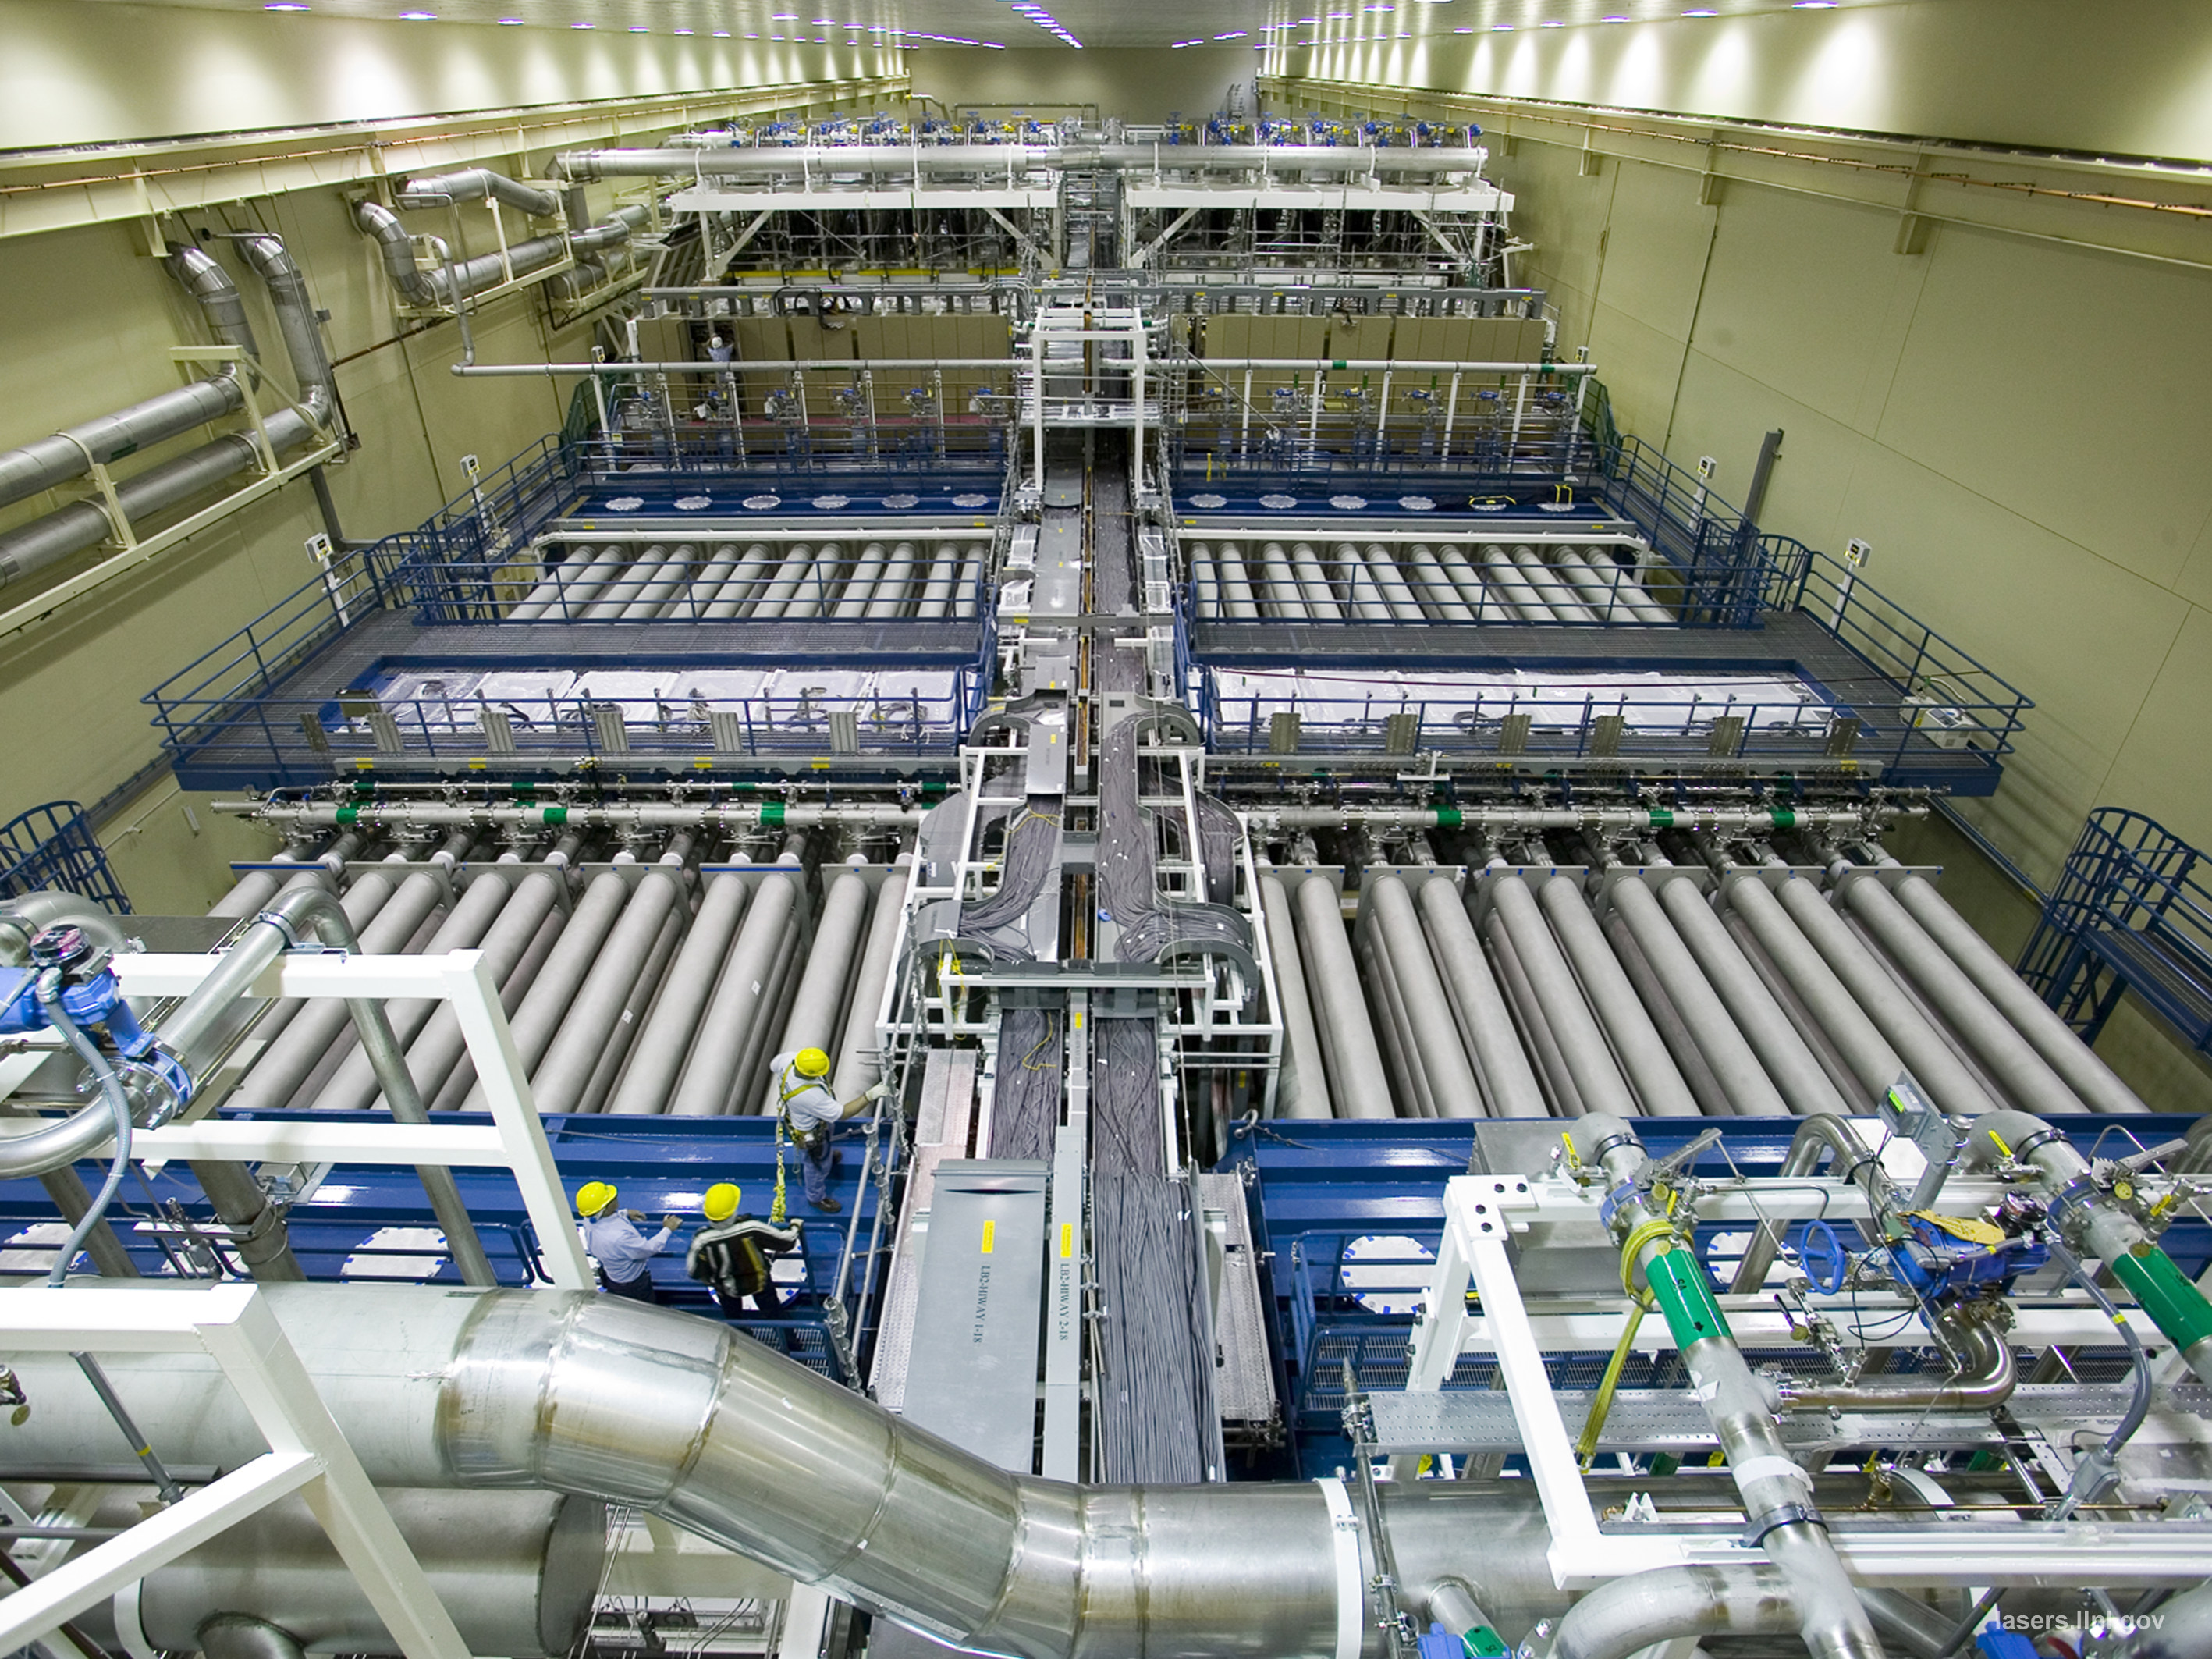
\includegraphics[width=80truemm]{slike/07_NIF_Laser_Bay.jpg}
\caption{Eden izmed najmočnejših laserskih sistemov na svetu, ki doseže 
$500~\si{\tera\watt}$ moči v sunku. \\Vir: National Ignition Facility, Livermore, Kalifornija.}
\label{fig:NIF}
\end{figure}

Laserski sistemi lahko oddajajo svetlobo z zelo veliko izhodno močjo. 
Najmočnejši zvezno delujoči laserji dosegajo moči 
$\sim 100~\si{\kilo\watt}$. Še bistveno večje moči dosegajo sunkovni laserji, 
saj lahko v sunku dosežejo moč tudi $\sim 500~\si{\tera\watt}$ (slika~\ref{fig:NIF}). 
Vendar so sunki s tako veliko svetlobno močjo izredno kratki, tipično reda pikosekunde, tako da
znaša celotna energija v sunku do nekaj $\si{\mega\joule}$. Pomemben
parameter pri sunkovnih laserjih je tudi čas, ki poteče med dvema zaporednima
sunkoma (repeticija). Najmočnejši laserski sistemi lahko izsevajo največ nekaj sunkov 
dnevno.\footnote{S. N. Dixit et al. CLEO: 2013, San Jose, CA (2013).}

\section{Helij-neonski laser}
\index{Laser!He-Ne}
Najprej si oglejmo helij-neonski (He-Ne) laser, ki je bil prvi zvezno 
delujoči laser in je še danes zelo razširjen.\footnote{A. Javan, W. R. Bennet Jr. in 
D. R. Herriott, Phys. Rev. Lett. $\mathbf{6}$, 106 (1961).} Najpogosteje deluje 
pri valovni dolžini $632,8~\si{\nano\metre}$ v rdečem delu spektra, lahko 
pa tudi pri infrardečih $1,15~\si{\micro\metre}$ in 
$3,39~\si{\micro\metre}$ ter nekaterih drugih\index{Infrardeče valovanje}
valovnih dolžinah v oranžnem in zelenem delu spektra. Laser deluje v zveznem 
načinu delovanja s tipičnimi močmi $0,5$--$100~\si{\milli\watt}$.\index{Energijski nivoji!He-Ne} \index{Trinivojski sistem}

Ojačevalno sredstvo je plin, mešanica helija in neona, katerih relevantni
energijski nivoji so prikazani na sliki~\ref{fig:HeNeE}. 
Atome helija
s trki z elektroni vzbudimo v eno izmed dveh dolgoživih metastabilnih stanj, 
to je $2^3$S ali
$2^1$S, z razpadnima časoma $0,1~\si{\milli\second}$ in $5~\si{\micro\second}$.
Ti dve stanji slučajno praktično sovpadata z dvema stanjema neona ($4$s in $5$s). 
Ko heliju dodamo neon, se energija s trki 
prenese z vzbujenih helijevih atomov na atome neona, ki s tem preidejo v 
že omenjeni vzbujeni stanji. Helijevi atomi se po trku vrnejo v osnovno stanje, od koder
jih ponovno vzbudimo. Prenos energije z atomov helija na atome neona s trki je 
zelo učinkovit, zato zasedenost vzbujenih neonovih stanj hitro naraste. Ko preseže 
zasedenost nižjih vzbujenih stanj, dosežemo obrnjeno zasedenost. 

Znana rdeča svetloba He-Ne laserja z valovno dolžino $632,8~\si{\nano\metre}$ nastane 
pri prehodu iz stanja $5$s v eno od stanj $3$p. Pri tem je življenjski čas 
stanja $5$s okoli $100~\si{\nano\second}$, stanja $3$p pa okoli $10~\si{\nano\second}$, zato
se spodnji nivo s spontano emisijo hitro prazni v metastabilno stanje $3$s. 
V tem stanju se atomi kopičijo, saj so dipolni sevalni prehodi v osnovno stanje prepovedani.
Atomi prehajajo v osnovno stanje le s trki ob steno cevi. Da pospešimo
praznjenje nivoja $3$s in omogočimo večjo obrnjeno zasedenost, zmanjšamo 
premer razelektritvene cevi. Zaradi gibanja atomov je spektralna 
črta Dopplerjevo razširjena\index{Dopplerjeva razširitev} ($\Delta \nu = 1,5~\si{GHz}$).
\begin{figure}[ht]
\centering
\def\svgwidth{95truemm} 
\input{slike/07_HeNeE.pdf_tex}
\caption{Shema energijskih nivojev v He-Ne laserju. Nivoji helija so označeni
z modro in nivoji neona z zeleno, laserski prehodi pa z rdečimi barvami in pripisano
ustrezno valovno dolžino.}
\vglue-5truemm
\label{fig:HeNeE}
\end{figure}

Laser deluje tudi pri prehodu iz stanja $5$s v stanje $4$p, pri katerem 
ima izsevana svetloba valovno dolžino $3,39~\si{\micro\metre}$. 
Ojačenje je za ta prehod celo precej večje kot za
prehod pri $632,8~\si{\nano\metre}$, deloma zaradi nižje frekvence 
(glej zvezo med Einsteinovima koeficientoma $A$ in $B$, enačba~\ref{4.27}), 
deloma zaradi kratke življenjske dobe spodnjega laserskega nivoja $4$p. 
Zato bi pričakovali, da bo He-Ne laser svetil v infrardečem delu in ne vidnem. 
To delno prepreči absorpcija v steklu, delno pa izgube namerno povečamo s selektivno odbojnostjo
resonatorskih zrcal, ki dvigne prag delovanja za $3,39~\si{\micro\metre}$ 
nad prag za $632,8~\si{\nano\metre}$. V laser lahko dodamo tudi
komoro metana, ki infrardeči del svetlobe močno absorbira, vidnega pa ne.
Omenimo še prehode iz stanja $4$s, ki ga dosežejo neonovi atomi s trki
z vzbujenimi helijevimi atomi iz nivoja $2^3$S. Prehod $4$s v $3$p, ki da svetlobo
pri $1,15~\si{\micro\metre}$, je bil prvi opažen prehod v He-Ne laserjih.
Zaradi razcepov posameznih nivojev je možnih prehodov še veliko več.

Tipičen He-Ne laser je razmeroma preprosto zgrajen (sliki~\ref{fig:HeNeShema}
in \ref{fig:Iskra}).\index{Laser!zgradba}
V razelektritveni cevi (napetost  $\sim 1~\si{\kilo\volt}$), skozi
katero teče električni tok ($\sim 10~\si{\milli\ampere}$), 
se nahaja mešanica helija in neona v razmerju od
$5:1$ do $10:1$. Skupni tlak v cevi je nizek, le okoli $3~\si{\milli\bar}$, 
cev pa je tipično dolga okoli $0,5~\si{\metre}$ s premerom $1$--$2~\si{\milli\metre}$.  
Cev s plinom na obeh straneh zapirata okni, ki sta nagnjeni za Brewstrov kot, 
tako da so izgube pri odboju za eno polarizacijo kar se da majhne.\index{Brewstrovo okno}
Izhodna svetloba iz laserja je zato polarizirana. V manjših laserjih
so namesto Brewstrovih oken na razelektritveno cev privarjena kar
resonatorska zrcala, zaradi česar so taki laserji nepolarizirani. 
Navadno je razelektritvena cev obdana z dvema ukrivljenima zrcaloma, 
ki imata zelo veliko odbojnost za izbrano valovno dolžino.
Nekaj tipičnih podatkov za He-Ne laser je zbranih v tabeli~\ref{tab:Ar}.

He-Ne laserji so preprosti, stabilni, zanesljivi, poceni, imajo visoko kakovost
snopa in dolgo služijo ($\sim~50\,\,000$ ur).
Danes jih sicer izrivajo polprevodniški laserji, vendar so še vedno v uporabi
v merilnih napravah, optičnih bralnih sistemih, šolah, raziskovalnih 
laboratorijih za interferometrijo in holografijo itd. Na njem je osnovan tudi 
standard za meter.
\newpage 

\begin{figure}[ht]
\centering
\def\svgwidth{90truemm} 
\input{slike/07_HeNeShema.pdf_tex}
\caption{Shema He-Ne laserja: R -- razelektritvena cev, IZ -- izhodno zrcalo, Z -- zrcalo
z veliko odbojnostjo, B -- Brewstrovi okni}
\label{fig:HeNeShema}
\end{figure}
\begin{figure}[ht]
\centering
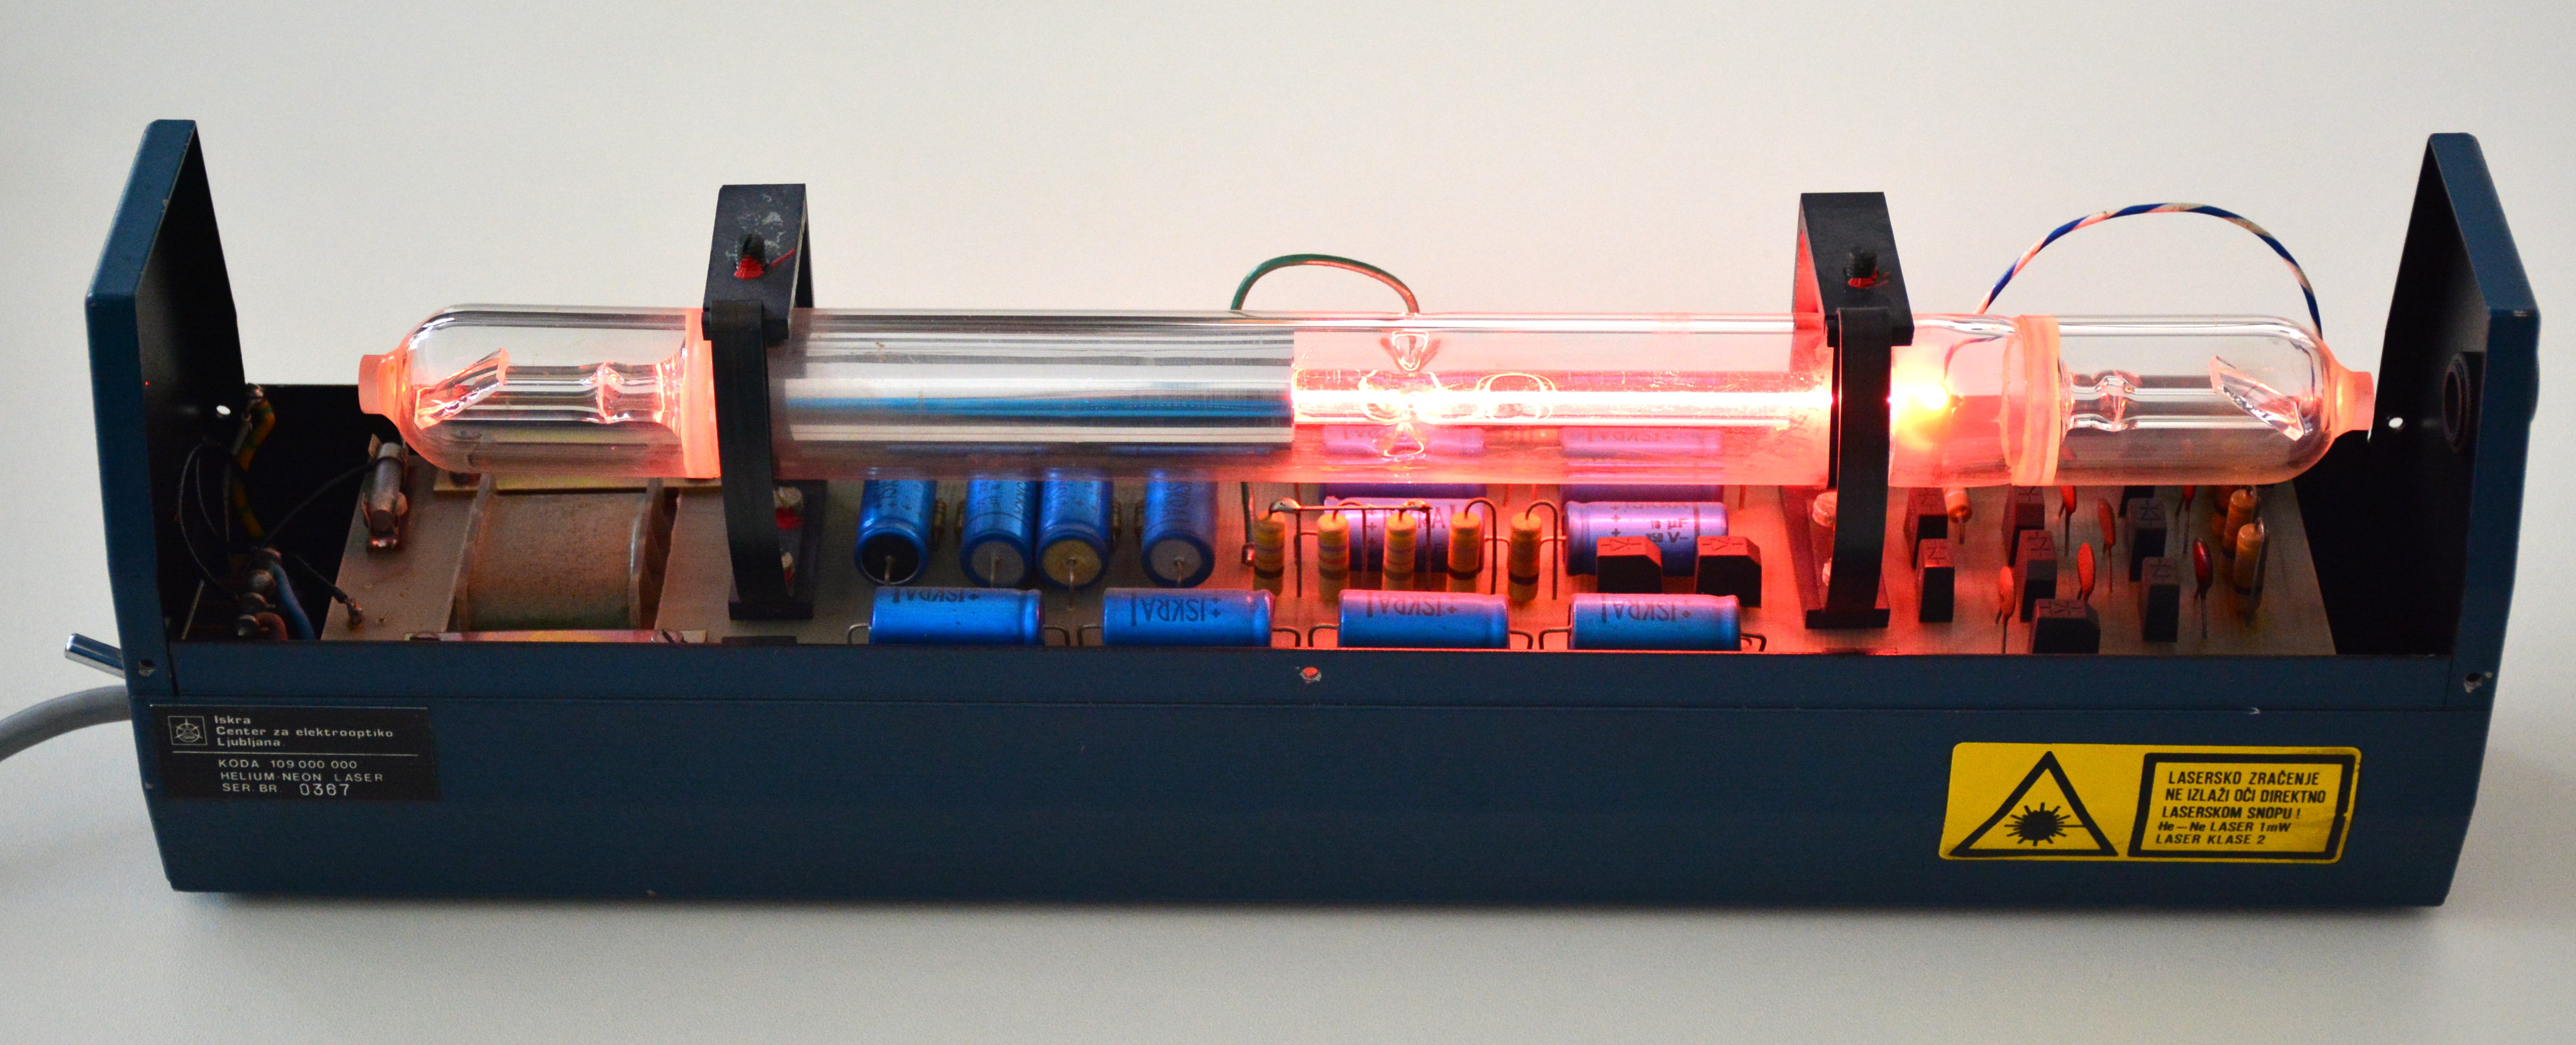
\includegraphics[width=128truemm]{slike/07_HeNe.jpg}
\caption{Primer starejšega He-Ne laserja, izdelanega v Sloveniji}
\label{fig:Iskra}
\end{figure}

\section{Argonski laser}
\index{Laser!argonski}
Kot drugi primer plinskega laserja obravnavajmo argonski laser ali natančneje
laser na argonove ione (Ar$^+$). Zanj je značilno zvezno 
delovanje v modrem in zelenem delu spektra pri 
valovnih dolžinah $488,0~\si{\nano\metre}$ in $514,5~\si{\nano\metre}$, deluje 
pa tudi v bližnjem ultravijoličnem delu spektra.\footnote{W. B. Bridges,
Appl. Phys. Lett. $\mathbf{4}$, 128 (1964).} Tipične moči delovanja argonskega laserja
so od $100~\si{\milli\watt}$ do $50~\si{\watt}$.\index{Ultravijolično valovanje}

Kot večino plinskih laserjev tudi tega črpamo z električnim tokom.
Atome argona vzbudimo s trki z elektroni v ione argona, ti pa z nadaljnjimi
trki preidejo v vzbujena stanja. Obrnjeno zasedenost
dosežemo med nivojema $4$p in $4$s (slika~\ref{fig:ArE}). 
Ta dva nivoja vsebujeta veliko podnivojev, zato je tudi prehodov med
njima zelo veliko. Argonski laser tako seva pri več kot tridesetih različnih
valovnih dolžinah, najznačilnejši sta že omenjeni 488~nm in 514,5~nm. 
Življenjski čas zgornjega nivoja je okoli $10~\si{ns}$, kar je približno 
desetkrat več od življenjskega časa spodnjega nivoja, od koder se ioni
z rekombinacijo z elektroni vrnejo v osnovno stanje. Tudi pri tem laserju
je poglavitni vzrok za razširitev črte \index{Dopplerjeva razširitev}Dopplerjev 
pojav ($\Delta \nu = 3,5~\si{GHz}$).\index{Energijski nivoji!argon}

Argonski laser je v osnovi zgrajen podobno kot He-Ne laser. \index{Laser!zgradba}
V razelektritveni cevi
(tipična dolžina $1~\si{\metre}$ in premer $1$--$2~\si{\milli\metre}$)
se nahaja argon pri pritisku okoli $10~\si{\milli\bar}$. 
Ker gre pri vzbujanju atomov argona za dvostopenjski proces, mora biti električni tok, 
s katerim dosežemo obrnjeno zasedenost, precej velik, lahko tudi nekaj deset amperov. 
Pri tipični napetosti nekaj kV to pomeni, 
da so za delovanje potrebne velike električne moči, 
pogosto več deset~$\si{\kilo\watt}$. Močnejši argonski laserji morajo biti
zaradi velike količine odvečne toplote hlajeni, najpogosteje vodno.
\vglue-2truemm
\begin{figure}[ht]
\centering
\def\svgwidth{75truemm} 
\input{slike/07_ArE.pdf_tex}
\caption{Shema energijskih nivojev v argonskem laserju}
\label{fig:ArE}
\end{figure}
\begin{figure}[ht]
\centering
\def\svgwidth{90truemm} 
\input{slike/07_ArShema.pdf_tex}
\caption{Poenostavljena shema argonskega laserja s prizmo: R -- razelektritvena cev, 
IZ -- izhodno zrcalo, Z -- zrcalo z veliko odbojnostjo, 
B -- Brewstrovi okni, \index{Brewstrovo okno} P -- prizma
}
\label{fig:ArS}
\end{figure}
\vglue-5truemm
\begin{remark}
V argonskih laserjih pogosto ustvarimo vzdolžno magnetno polje, ki preprečuje 
elektronom, da bi predčasno zapustili ojačevalno območje in trčili ob steno. S
tem se poveča izhodno moč laserja, hkrati pa preprečuje poškodbe na stenah, ki bi jih 
povzročili visokoenergijski elektroni. Iz istega razloga so pri močnejših
laserjih zrcala izven plinske cevi. 
\end{remark}
\vglue-3truemm
V resonator argonskega laserja moramo vgraditi še element, ki omogoči
izbiro ene same spektralne črte. Najpogosteje za ta frekvenčno selektiven element
uporabimo kar majhno prizmo pred enim od obeh zrcal (slika~\ref{fig:ArS}). Zaradi disperzije
v prizmi se snopi različnih valovnih dolžin lomijo pod različnimi koti in le tisti 
snop, ki vpada pravokotno na zrcalo, se ojačuje. Tako z vrtenjem prizme ali zrcala 
izbiramo valovno dolžino izhodne svetlobe. Nekaj tipičnih podatkov za argonski
laser je zbranih v tabeli~\ref{tab:Ar}.

Argonski laserji so zanesljivi in dajejo zelo dober osnovni Gaussov snop pri eni
sami frekvenci. Uporabljajo se v optični spektroskopiji,
interferometriji, holografiji in merilni tehniki. Delujejo v zveznem načinu,
zaradi razmeroma široke črte ojačenja jih uporabljamo tudi za fazno uklenjene
sunkovne laserje z dolžino sunkov okoli $150~\si{\pico\second}$. 
V kombinaciji s kriptonskimi laserji, ki so zelo podobni argonskim, le da delujejo
v rdečem in oranžnem delu spektra, se uporabljajo tudi v zabavni industriji.
V zadnjem času jih vse bolj izrivajo polprevodniški laserji in frekvenčno
podvojeni Nd:YAG laserji. 

\section{Laser na ogljikov dioksid}
\index{Laser!CO$_2$}
Osnova za delovanje do zdaj opisanih plinskih laserjev so elektronski prehodi
v atomih ali ionih. Osnova za delovanje laserja na ogljikov dioksid pa so 
prehodi med vibracijskimi stanji molekul 
CO$_2$, pri čemer elektroni ostanejo v osnovnem stanju.\footnote{C. K. N. Patel,
Phys. Rev. $\mathbf{136}$, A1187 (1964).}
Zaradi majhnih energijskih razlik med vibracijskimi stanji deluje
ta laser v infrardečem delu spektra, najpogosteje pri \index{Infrardeče valovanje}
$9,6~\si{\micro\metre}$ in $10,6~\si{\micro\metre}$. Laser deluje v zveznem
in sunkovnem načinu. Odlikujejo ga zelo velik izkoristek ($\sim 30~\%$) in 
posledično zelo velike moči, tipično od $1~\si{\watt}$ do $10~\si{\kilo\watt}$. 

Preden opišemo delovanje laserja, si na kratko oglejmo lastna nihanja molekule 
ogljikovega dioksida. Molekula CO$_2$ je v osnovnem stanju linearna molekula 
(slika~\ref{fig:CO2}\,a). 
Za molekule take oblike obstajajo trije osnovni načini nihanja atomov glede na težišče:
upogib, pri katerem atomi nihajo v smeri pravokotno na os (slika~\ref{fig:CO2}\,b),
simetrični razteg, pri katerem atoma kisika nihata simetrično vzdolž osi molekule, ogljik pa pri tem miruje (slika~\ref{fig:CO2}\,c), in asimetrični razteg, pri 
katerem atoma kisika nihata v isti smeri vzdolž osi, ogljik pa v nasprotni 
(slika~\ref{fig:CO2}\,d). Najvišjo frekvenco nihanja ima asimetrični razteg,
najnižjo pa upogib. 

Vsako vibracijsko stanje molekule lahko razstavimo na osnovne nihajne načine in 
ga opišemo s številom energijskih kvantov v posameznem osnovnem nihanju, 
torej s trojico celih števil $(n_1,n_2,n_3)$. Po dogovoru stanje 100 opisuje
osnovni simetrični razteg, stanje 010 osnovni upogib in stanje 001 
osnovni asimetrični razteg.

\begin{figure}[ht]
\centering
\def\svgwidth{110truemm} 
\input{slike/07_CO2.pdf_tex}
\caption{Molekula CO$_2$ (a) in trije osnovni načini nihanja molekule:
upogib (b), simetrični razteg~(c) in asimetrični razteg (d). Atomi ogljika so
označeni s črno
in kisika z rdečo barvo.}
\label{fig:CO2}
\end{figure}
\newpage

Vibracijska stanja molekule vzbudimo z električnim tokom skozi plin. 
\index{Energijski nivoji!CO$_2$}
Zato v razelektritveno cev dodamo dušik (N$_2$) in podobno kot pri He-Ne laserju
se tudi CO$_2$ črpa predvsem preko trkov z dušikovimi molekulami. 
Dušikova molekula je dvoatomna in ima zato zgolj eno vibracijsko stanje, ki po energiji
praktično sovpada z energijo stanja 001 (slika~\ref{fig:CO2E}). Iz tega zgornjega
nivoja molekule prehajajo v stanje 100 ($10,6~\si{\micro\metre}$) ali stanje
020 ($9,6~\si{\micro\metre}$). Da pospešimo prehod nazaj v osnovno stanje, 
plinski mešanici dodamo helij, s katerim trkajo molekule.
Razmerje parcialnih tlakov je navadno 1\,:\,1\,:\,8 za CO$_2$\,:\,N$_2$\,:\,He pri tlaku $1~\si{\milli\bar}$. 
Pri tako nizkih tlakih je poglavitna razširitev spektralne črte Dopplerjeva, 
\index{Dopplerjeva razširitev}ki 
je v primerjavi z ostalimi plinskimi laserji zaradi nizkih frekvenc zelo majhna,
le okoli $70~\si{\mega\hertz}$. V laserjih z višjim tlakom 
prevlada razširitev zaradi medmolekulskih trkov. Pri tlakih okoli $20~\si{\bar}$
znaša razširitev okoli $500~\si{\giga\hertz}$, kar omogoča izdelavo fazno uklenjenih 
sunkovnih laserjev s sunki dolžine $\sim 1~\si{\pico\second}$. Nekaj tipičnih podatkov 
za laser na ogljikov dioksid je zbranih v tabeli~\ref{tab:Ar}.
\vglue-1truemm
\begin{figure}[ht]
\centering
\def\svgwidth{90truemm} 
\input{slike/07_CO2E.pdf_tex}
\caption{Shema vibracijskih nivojev v laserju na ogljikov dioksid. 
Nivoji dušika so označeni z modro in nivoji CO$_2$ z zeleno, laserski prehodi 
pa z rdečimi barvami in pripisano valovno dolžino.}
\label{fig:CO2E}
\end{figure}
\vglue-2truemm
Najpreprostejši laser na ogljikov dioksid \index{Laser!zgradba} 
je po svoji zgradbi podoben drugim plinskim laserjem. 
Razelektritvena cev (polmer $\sim 1~\si{\centi\metre}$ 
in dolžina $0,5$--$2~\si{\metre}$) 
je na obeh koncih zaključena z Brewstrovima oknoma in zrcaloma. Vsi optični elementi
v laserju morajo biti seveda prepustni oziroma odbojni za infrardeči del spektra. Ker lahko 
laser deluje pri različnih valovnih dolžinah, dodamo v resonator frekvenčno selektiven
člen, na primer uklonsko mrežico (slika~\ref{fig:CO2S}).\index{Uklonska mrežica}
\vglue-4truemm
\begin{figure}[ht]
\centering
\def\svgwidth{90truemm} 
\input{slike/07_CO2Shema.pdf_tex}
\caption{Poenostavljena shema  laserja na ogljikov dioksid: R -- razelektritvena cev, 
IZ -- izhodno zrcalo, Z -- zrcalo z veliko odbojnostjo, B -- Brewstrovi okni, 
U -- uklonska mrežica\index{Brewstrovo okno}
}
\label{fig:CO2S}
\end{figure}

Laserji na ogljikov dioksid se zaradi svoje velike izhodne moči uporabljajo v 
industriji za zahtevne obdelave materialov, na primer za rezanje 
kovin, vrtanje, ablacijo, varjenje in tudi za vojaške namene. Zaradi velike
absorpcije izsevane svetlobe v vodi se uporabljajo tudi v medicinske namene, predvsem
za rezanje tkiv in dermatologijo. 
Obdelava z laserji omogoča veliko natančnost, čistočo in je zelo fleksibilna.

\begin{table}
% \footnotesize
\small
\begin{center}
\setlength\tabcolsep{4pt}
\begin{tabular}{|l|c|c|c|c|}\hline
Laser & He-Ne & Ar$^+$ & CO$_2$ & ekscimer\\ \hline
Valovna dolžina  $\lambda$ & $632,8~\si{\nano\metre}$& $488$ in
$514,5~\si{\nano\metre}$ & $9,6$ in $10,6~\si{\micro\metre}$ & UV
\\ \hline
Verjetnost za spontani prehod $A$ & $3,4 \times 10^6/\si{\second}$ & 
$7,8 \times 10^7/\si{\second}$ & $0,25/\si{\second}$ & $\sim 10^8/\si{\second}$ \\ \hline
Presek za stimulirano emisijo $\sigma$ & $3 \times 10^{-17}~\si{\metre}^2$&  $2,6 \times 10^{-16}~\si{\metre}^2$ & $3 \times 10^{-22}~\si{\metre}^2$ & $ 10^{-20}~\si{\metre}^2$ \\ \hline
Spektralna širina črte $\Delta \nu$ & $1,5 \times 10^{9}~\si{\hertz}$ & 
$3,5 \times 10^{9}~\si{\hertz}$ &$7 \times 10^{7}~\si{\hertz}$ & $10^{13}~\si{\hertz}$ \\ \hline
Obrnjena zasedenost $\Delta N/V$ & $5 \times 10^{15}/\si{\metre}^3$ & $2 \times 10^{15}/\si{\metre}^3$ & $3 \times 10^{21}/\si{\metre}^3$ & $10^{20}/\si{\metre}^3$\\ \hline
\end{tabular}
\caption{Izbrani podatki za helij-neonski laser, argonski laser, laser na ogljikov dioksid in tipičen ekscimerni laser}
\index{Laser!He-Ne}
\index{Laser!argonski}
\index{Laser!CO$_2$}
\index{Laser!ekscimerni}
\label{tab:Ar}
\end{center}
\end{table}

\section{Ekscimerni laser}
\index{Laser!ekscimerni}
Beseda ekscimer ({\it excited dimer, excimer}) označuje vzbujena vezana 
stanja dveh atomov, 
ki se v osnovnem stanju ne bi vezala.\footnote{N. G. Basov et al., JETP Lett.
$\mathbf{12}$, 329 (1970).}
Za laserje so zanimivi predvsem ekscimeri
težkih žlahtnih plinov in halogenov, na primer Ar$_2^*$ ($126~\si{\nano\metre}$), 
Kr$_2^*$ ($146~\si{\nano\metre}$), Xe$_2^*$ ($172~\si{\nano\metre}$),
ArF ($193~\si{\nano\metre}$), KrF ($248~\si{\nano\metre}$), 
XeCl ($308~\si{\nano\metre}$), ArBr ($161~\si{\nano\metre}$) in 
NeF ($108~\si{\nano\metre}$). Te molekule obstajajo samo v vzbujenem stanju,
v osnovnem stanju  je zaradi prevelike odbojne sile med atomoma molekula neobstojna.
Vsi našteti primeri oddajajo lasersko svetlobo v\index{Ultravijolično valovanje}
ultravijoličnem delu, ki ga drugi laserski sistemi le težko pokrivajo. 
Ekscimerni laserji delujejo v sunkih, pri čemer je tipična oddana energija v sunku 
$\sim 1~\si{\joule}$, dolžina sunka pa $10$--$100~\si{\nano\second}$ pri repeticiji
$\sim 100~\si{\hertz}$.

Dva atoma se vežeta, kadar je ionizacijska energija prvega
atoma manjša od vsote elektronske afinitete drugega atoma in
elektrostatične energije vezave obeh ionov. Vzemimo za primer klor in
kripton. Ionizacijska energija kriptona v osnovnem stanju je 14~eV, v
vzbujenem pa 5~eV. Elektronska afiniteta klora je 3,75~eV in
elektrostatična vezavna energija KrCl okoli 7~eV. Tako je treba za nastanek
molekule KrCl v osnovnem stanju dodati okoli 4~eV, pri tvorbi
molekule v vzbujenem stanju pa se sprosti okoli 6~eV. Odvisnost
potencialne energije molekule KrCl v osnovnem in vzbujenem stanju
kaže slika~\ref{fig:exE}. Molekula, ki je vezana v vzbujenem stanju, po
sevalnem prehodu v osnovno stanje takoj razpade, zato je zelo lahko doseči
obrnjeno zasedenost. Razpadni čas vezanega stanja je $\sim~10~\si{\nano\second}$ in
spodnjega nevezanega okoli $0,1~\si{\pico\second}$.
Da nastanejo ekscimeri, vzbujamo mešanico 
plinov v heliju. Pritisk
je razmeroma velik ($\sim 3~\si{\bar}$), zato plin v cevi vzbujamo prečno.
Velika je tudi spektralna širina prehoda ($\Delta\nu = 10^{13}~\si{Hz}$). Nekaj tipičnih podatkov 
za ekscimerne laserje je zbranih v tabeli~\ref{tab:Ar}.
\index{Energijski nivoji!ekscimer}

Ekscimerni laserji delujejo v sunkih s precej 
veliko energijo in se zaradi kratke valovne
dolžine in velike natančnosti uporabljajo v 
fotolitografiji in izdelavi mikroprocesorjev 
ter medicini, predvsem oftalmologiji in kirurgiji.
\begin{figure}[ht]
\centering
\def\svgwidth{45truemm} 
\input{slike/07_exE.pdf_tex}
\caption{Shema energije $E$ v odvisnosti od razdalje med jedroma atomov $d$. 
V vzbujenem stanju
se atoma povežeta v molekulo, po prehodu v nižji nivo  molekula razpade.}
\label{fig:exE}
\end{figure}

\section{Neodimski laser}
Druga skupina laserjev, ki jo bomo obravnavali, so trdninski laserji. Taki laserji
temeljijo na elektronskih prehodih v ionih primesi, ki jih dodamo v kristal ali steklo,
črpamo pa jih optično. Primesi so navadno redke zemlje ali prehodne kovine, 
kristali pa so oksidi ali fluoridi. Izdelava ojačevalnih sredstev na osnovi stekla
je bistveno preprostejša in cenejša, vendar ima steklo precej nižjo toplotno prevodnost
od kristalov in se zato bolj greje. 
Začeli bomo z opisom dveh primerov neodimskega laserja, Nd:YAG
in Nd:steklo.\footnote{
Podobne laserje dobimo, če v kristalu YAG itrijeve ione deloma
nadomestimo z iterbijem ($1030~\si{\nano\metre}$) ali 
erbijem ($2940~\si{\nano\metre}$).\index{Iterbij}\index{Erbij}} 
\vglue-4truemm
\subsection{Nd:YAG}
\index{Laser!Nd:YAG}
V Nd:YAG laserju\footnote{J. E. Geusic,
H. M. Marcos in L. G. Van Uitert, Appl. Phys. Lett. $\mathbf{4}$, 182 (1964).} je ojačevalno sredstvo
itrij-aluminijev granat (Y$_3$Al$_5$O$_{12}$, YAG) s primesmi neodimovih ionov Nd$^{3+}$. 
Laser deluje pri valovni dolžini $1,064~\si{\micro\meter}$ ali frekvenčno podvojeni
$532~\si{\nano\metre}$. Deluje v zveznem \index{Infrardeče valovanje}
načinu pri močeh do $5~\si{\kilo\watt}$ ali sunkovnem z dolžino sunkov okoli 
$100~\si{\nano\second}$ in energijo sunka $\sim 1~\si{\joule}$.

Neodimski laser je primer štirinivojskega laserja, 
\index{Štirinivojski sistem}pri čemer je 
laserski prehod med stanjema $^4$F$_{3/2}$ in $^4$I$_{11/2}$ neodimovih ionov 
(slika~\ref{fig:NdE}). S svetlobo z valovno dolžino tipično 
okoli $800~\si{\nano\metre}$ črpamo elektrone v višje nivoje, ki hitro 
preidejo v zgornji laserski nivo. Življenjski čas zgornjega nivoja je 
okoli $230~\si{\micro\second}$, spodnjega pa precej krajši, zato je 
lahko doseči veliko obrnjeno zasedenost. Spodnje stanje je dovolj visoko nad 
osnovnim, da pri sobni temperaturi v ravnovesju ni znatno zasedeno. 
Razširitev črte je homogena in je posledica predvsem \index{Spektralna črta!homogena razširitev}
termičnega nihanja kristalne mreže ($\Delta \nu = 130~\si{GHz}$). 
Prag neodimskega laserja za zvezno delovanje je nizek in ga je lahko doseči, 
prav tako dobro neodimski laser deluje v sunkih, predvsem s preklopom dobrote.
\index{Energijski nivoji!Nd:YAG}

\begin{figure}[ht]
\centering
\def\svgwidth{95truemm} 
\input{slike/07_NdE.pdf_tex}
\caption{Shema energijskih nivojev neodimovih ionov v Nd:YAG laserju}
\label{fig:NdE}
\end{figure}
Laser optično črpamo z diodnimi laserji 
ali močnimi ksenonskimi svetilkami za zvezno delovanje 
in podobnimi bliskavicami za sunkovno delovanje (slika~\ref{fig:Nd}\,a). 
Aktivna snov v laserju je v obliki paličice dolžine od nekaj cm do dobrih 
$10~\si{\centi\metre}$ in premera $\sim 1~\si{\centi\metre}$. 
V kristalu YAG neodimovi ioni nadomestijo približno $1~\%$ itrijevih, zato je ojačevalno
sredstvo na videz rahlo rožnato (slika~\ref{fig:Nd}\,b). 
Aktivna paličica in svetilka sta vgrajeni v cilindrično ali eliptično votlino z 
zrcalnimi ali belimi stenami, tako da se čim večji del črpalne svetlobe absorbira v 
laserski paličici (slika~\ref{fig:Nd}\,c).

\begin{figure}[ht]
\centering
\def\svgwidth{128truemm} 
\input{slike/07_Nd.pdf_tex}
\caption{Ksenonska bliskavica (a), ojačevalno sredstvo v Nd:YAG laserju (b) 
in shema prečnega preseka eliptične črpalne votline (c)}
\label{fig:Nd}
\end{figure}

Pri črpanju s ksenonsko svetilko je le manjši del črpalne svetlobe v
absorpcijskih pasovih, zato je izkoristek razmeroma slab, tipično 
pod $1~\%$. Za izhodno moč zvezno delujočega Nd:YAG laserja $\sim 10~\si{\watt}$ je tako
potrebna električna moč $\sim 1~\si{kW}$. Velika večina porabljene moči 
gre v gretje, zato je v laserjih z nekoliko večjo povprečno
močjo potrebno vodno hlajenje. Gretje povzroča tudi toplotne deformacije
laserske paličice, kar lahko močno spremeni lastnosti resonatorja. Toplotni
učinki so poglavitna praktična težava pri izdelavi neodimskih
laserjev s klasičnimi svetilkami. Danes zato zvezno delujoče neodimske laserje
črpamo z diodnimi laserji, ki svetijo v območju največje
absorpcije Nd$^{3+}$. Črpanje je lahko prečno ali vzdolžno (slika~\ref{fig:NdS}). 
Pri diodnem črpanju je izkoristek dosti večji in je manj gretja, kar omogoča 
bolj kompaktno konstrukcijo in boljšo stabilnost izhodne moči.
\index{Laser!zgradba} 
\begin{figure}[ht]
\centering
\def\svgwidth{120truemm} 
\input{slike/07_NdS.pdf_tex}\index{Črpanje!vzdolžno}
\caption{Shema vzdolžno črpanega Nd:YAG laserja: O -- ojačevalno sredstvo, 
IZ -- izhodno zrcalo, D -- dikroično zrcalo, 
prepustno za črpalno svetlobo in odbojno za lasersko, DL -- diodni 
laser za črpanje, L -- leča
}
\label{fig:NdS}
\end{figure}

Neodimski laserji so zelo razširjeni, tako v osnovni kot v frekvenčno 
podvojeni različici. Uporabni so za obdelavo materialov (vrtanje, varjenje, 
litografija). Ker snop preprosto sklopimo v optično vlakno, so 
zelo uporabni tudi v medicini (endoskopska kirurgija in dermatologija). 
Pomemben proizvajalec sunkovnih Nd:YAG laserjev 
za medicinske namene je podjetje Fotona, d.\,o.\,o., iz Ljubljane.\index{Fotona d.o.o.}

\begin{table}[ht]
\small
\begin{center}
\begin{tabular}{|l|c|c|c|}\hline
Laser & Nd:YAG & Nd:steklo & Ti:safir \\ \hline
Valovna dolžina  & $1064~\si{\nano\metre}$ & $1050~\si{\nano\metre}$ & 
 $600-1100~\si{\nano\metre}$\\ \hline
Verjetnost za spontani prehod $A$ & $4 \times 10^3/\si{\second}$ & $3 \times 10^3/\si{\second}$
& $3 \times 10^5/\si{\second}$\\ \hline
Presek za stimulirano emisijo $\sigma$ & $3 \times 10^{-23}~\si{\metre}^2$ &
$3 \times 10^{-24}~\si{\metre}^2$ & $3 \times 10^{-23}~\si{\metre}^2$\\ \hline
Spektralna širina črte $\Delta \nu$ & $1,3 \times 10^{11}~\si{\hertz}$ &
$7 \times 10^{12}~\si{\hertz}$ & $1 \times 10^{14}~\si{\hertz}$\\ \hline
Gostota obrnjene zasedenosti $\Delta N/V$ & $1,6 \times 10^{23}/\si{\metre}^3$ &
$8 \times 10^{23}/\si{\metre}^3$ & $6 \times 10^{23}/\si{\metre}^3$\\ \hline
\end{tabular}
\caption{Tipični podatki za Nd:YAG, Nd:steklo in Ti:safirni laser}
\index{Laser!Nd:YAG}
\index{Laser!Nd:steklo}
\index{Laser!Ti:safir}
\label{tab:nd}
\end{center}
\end{table}

\subsection{Nd:steklo}
\index{Laser!Nd:steklo}
Namesto v kristal lahko neodimove ione Nd$^{3+}$ vgradimo tudi v steklo. 
Laser z ojačevalnim sredstvom Nd:steklo  deluje 
pri valovni dolžini $1,050~\si{\micro\meter}$ v sunkovnem načinu 
s preklopom dobrote ali z uklepanjem faz z energijami sunkov $~\sim 1~\si{\joule}$.
Zaradi amorfne strukture stekla in posledično 
nehomogenega lokalnega polja je laserska črta nehomogeno razširjena in
razmeroma široka ($\Delta\nu=7~\si{THz}$).
\index{Spektralna črta!nehomogena razširitev}

Ojačenje je manjše kot v Nd:YAG in za prag laserskega delovanja je
potrebna precej večja črpalna moč. Laserji z ojačevalnim sredstvom 
Nd:steklo se zato uporabljajo le v 
sunkovnem načinu in za tako delovanje so celo primernejši od Nd:YAG laserjev.
Zaradi manjšega ojačenja pri dani obrnjeni zasedenosti 
je v laserju s preklopom dobrote mogoče doseči večjo načrpanost, 
preden pride do praznjenja
zaradi ojačevanja spontanega sevanja v enem preletu paličice. 

Problem teh laserjev
predstavlja nizka toplotna prevodnost stekla, ki omejuje repeticijo sunkov.
Velika širina spektralne črte je zelo primerna za delovanje v načinu uklepanja faz, s 
katerim dosegamo ultrakratke sunke ($\sim 100~\si{\femto\second}$). 

\begin{remark}
Energije izsevanih sunkov je mogoče še povečati z ojačevalniki. Med največjimi je
laserski sistem Nd:steklo, ki ga uporabljajo za raziskave fuzije (NIF -- National Ignition Facility, 
Livermore, Kalifornija).
Okoli $1~\si{\nano\second}$ dolg sunek iz osnovnega laserja razdelijo na 192
ojačevalnih vej, ga postopoma ojačujejo in nato na koncu spet združijo.
Končna energija sunka je tako nad $\sim 1~\si{\mega\joule}$. Z njim z vseh strani posvetijo na
kroglico iz devterija in tritija, ki se dovolj segreje in stisne, da pride do 
njunega zlivanja. Vršna moč laserskega sunka je okoli $10^{15}$~W. 
Če laserski snop zberemo na površino 1~mm$^2$, je v gorišču jakost električnega polja
okoli $5 \times 10^{11}$~V/m, kar je približno enako električnemu polju v vodikovem atomu.
\end{remark}

\section{Titan-safirni laser}
\index{Laser!Ti:safir}
Titan-safirni (Ti:safir) 
laser je trdninski laser\footnote{P. F. Moulton, J. Opt. Soc. Am. B $\mathbf{3}$
125 (1986).}, pri katerem so v kristal safirja
Al$_2$O$_3$ primešani ioni titana Ti$^{3+}$. Njegova najpomembnejša značilnost je
zvezna nastavljivost valovne dolžine v zelo širokem frekvenčnem pasu 
($600$--$1100~\si{\nano\metre}$) z največjo učinkovitostjo pri okoli $800~\si{\nano\metre}$. Deluje
v zveznem načinu z močmi do $50~\si{\watt}$ in sunkovno  v fazno uklenjenem načinu 
z dolžino sunkov $\sim~10~\si{\femto\second}$ z vršnimi močmi nad $10^{12}~\si{\watt}$. 
\index{Energijski nivoji!Ti:safir}
\begin{figure}[ht]
\centering
\def\svgwidth{70truemm} 
\input{slike/07_TiE.pdf_tex}
\caption{Energijski nivoji v Ti:safir laserju. Nivoja sta zaradi vibracij
razcepljena na veliko število podnivojev, ki se med seboj deloma prekrivajo.
}
\label{fig:TiE}
\end{figure} 

Ojačevalno sredstvo v Ti:safir laserju je aluminijev oksid, v katerem 
približno $0,2~\%$ aluminijevih ionov nadomestimo s titanovimi. Titanovi ioni imajo 
v taki konfiguraciji zgolj eno vzbujeno stanje, vendar se zaradi sklopitve s fononi
vibracijski nivoji posameznega stanja med seboj prekrivajo in prehod je močno razširjen. 
Z optičnim črpanjem vzbudimo titanove ione iz osnovnega stanja v eno izmed vibracijskih 
stanj vzbujenega stanja. Ioni nato hitro preidejo v najnižje vzbujeno stanje. 
Laserski prehod poteka med najnižjim vzbujenim stanjem in enim od vibracijskih 
nivojev osnovnega stanja (slika~\ref{fig:TiE}). Življenjski čas
vzbujenega stanja je kratek ($3,2~\si{\micro\second}$) in širina črte največja med
vsemi trdninskimi laserji ($\Delta \nu =  100~\si{THz}$). 
Ker je vrh absorpcijskega pasu blizu $500~\si{\nano\metre}$,
laser črpamo z zeleno svetlobo (argonski laser oziroma
frekvenčno podvojen neodimski laser za sunkovno delovanje). 
Najpomembnejša uporaba Ti:safir laserjev je v raziskovalnih laboratorijih za ustvarjanje zelo 
kratkih sunkov svetlobe z dolžino $\sim 10~\si{\femto\second}$. Pot, ki jo 
v tem času prepotuje svetloba, je le nekaj valovnih dolžin svetlobe. 

\section{Laserji na organska barvila}
\index{Laser!organska barvila}
V laserjih na organska barvila je barvilo raztopljeno v tekočini, praviloma vodi ali alkoholu. 
To so bili prvi laserji z veliko spektralno širino in nastavljivo valovno dolžino
izhodne svetlobe. Delujejo lahko kot zvezni laserji in z izbiro barvila dosežemo
delovanje v območju $300$--$1500~\si{\nano\metre}$ pri močeh do $\sim 2~\si{\watt}$.
Široka spektralna širina omogoča sunkovno delovanje z uklepanjem faz. Dolžina 
sunkov je nekaj femtosekund, energija v sunkih pa nekaj $100~\si{\joule}$.

Shema energijskih nivojev molekule tipičnega organskega barvila
je zelo podobna shemi energijskih nivojev Ti:safir laserja (slika~\ref{fig:TiE}).
Vsi elektronski nivoji so razcepljeni v vibracijske in rotacijske podnivoje. 
V toplotnem ravnovesju je molekula na dnu osnovnega elektronskega stanja S$_0$. 
Z absorpcijo vidne svetlobe primerne frekvence preide v neko vzbujeno
singletno stanje S$_1$. Prek trkov z molekulami topila vzbujena barvilna molekula
zelo hitro, v času okoli pikosekunde, preide na dno vzbujenega stanja, od
koder s sevanjem preide nekam v osnovno stanje S$_0$, od tam pa s trki
hitro nazaj na dno osnovnega stanja. Ker
sta obe elektronski stanji zaradi vibracij in rotacij razširjeni, sta 
absorpcijska in emisijska fluorescenčna črta široki ($\Delta \nu = 30~\si{THz}$).
Energija izsevane svetlobe je zmanjšana za energijo
prehodov s trki, zato je emisijska črta premaknjena k nižjim
frekvencam glede na absorpcijsko. Absorpcijski in fluorescenčni 
spekter prehoda S$_0-$S$_1$
za barvilo rodamin 6G kaže slika~\ref{fig:RhG}.

Laser na organska barvila lahko deluje pri vseh frekvencah znotraj široke
fluorescenčne črte. Zato moramo v resonator vgraditi frekvenčno
selektivni element, s katerim nastavljamo frekvenco izhodne svetlobe. Za to lahko 
uporabimo prizmo ali eno od zrcal nadomestimo 
z uklonsko mrežico, ki je zasukana pod takim kotom, da se po osi resonatorja odbije le svetloba
izbrane valovne dolžine.\index{Uklonska mrežica}
Barvilne laserje črpamo ali z bliskavico ali z drugim laserjem primerne 
valovne dolžine, na primer argonskim ali ekscimernim.

\begin{figure}[ht]
\centering
\def\svgwidth{70truemm} 
\input{slike/07_RhG.pdf_tex}
\caption{Absorpcijski in emisijski spekter barvila rodamin 6G, ki se uporablja v laserjih}
\label{fig:RhG}
\end{figure} 
\begin{table}[ht]
\begin{center}
\begin{tabular}{|l|c|}\hline
Valovna dolžina  & $300$--$1500~\si{\nano\meter}$\\ \hline
Verjetnost za spontani prehod $A$ & $ \sim 10^8/\si{\second}$ \\ \hline
Presek za stimulirano emisijo $\sigma$ & $3 \times 10^{-20}~\si{\metre}^2$ \\ \hline
Spektralna širina črte $\Delta \nu$ & $3 \times 10^{13}~\si{\hertz}$  \\ \hline
Gostota obrnjene zasedenosti $\Delta N/V$ & $ \sim 10^{22}/\si{\metre}^3$ \\ \hline
\end{tabular}
\caption{Tipični podatki za laserje na organska barvila}
\label{tab:orgb}
\end{center}
\end{table}
\vglue-5truemm
Slabost laserjev na organska barvila je njihova degradacija. Barvila v
laserjih je treba pogosto menjati (tipično na 100 ur delovanja), poleg tega je ravnanje
z njimi zahtevno, saj je veliko barvil in topil strupenih ali korozivnih.
Laserji na organska barvila so zaradi svoje nastavljive valovne dolžine
uporabni v spektroskopiji, za ločevanje izotopov, v 
medicini (dermatologija, odstranjevanje ledvičnih kamnov) itd.
 
\section{Vlakenski laserji}
\index{Laser!vlakenski}
Posebna vrsta laserjev so vlakenski laserji, v katerih za aktivno 
sredstvo uporabimo optično vlakno, dopirano z ioni \index{Optično vlakno}redkih zemelj.\footnote{~Za
podroben opis optičnih vlaken glej poglavje~\ref{chap:fibri}.}
Valovna dolžina, pri kateri oddajajo svetlobo, je odvisna od snovi, s katerimi
je vlakno dopirano. Najpogosteje je to erbij ($1550~\si{nm}$),\index{Erbij}
iterbij ($\sim 1100~\si{nm}$)\index{Iterbij} ali neodim ($1064~\si{nm}$).
Vlakenske laserje odlikujeta \index{Infrardeče valovanje}
izredno velik izkoristek (tipično okoli $70$--$80~\%$, lahko tudi več) 
in posledično zelo velika moč (do $20~\si{kW}$). Zanje sta značilni tudi
izredno velika kakovost snopa (faktor $M^2<1,1$, glej 
razdelek~\ref{chap:gaussovsnop}) in 
razmeroma majhna občutljivost na zunanje motnje. Delujejo lahko v zveznem
ali sunkovnem načinu.\index{Faktor $M^2$}

\begin{figure}[ht]
\centering
\def\svgwidth{110truemm} 
\input{slike/07_FibEr.pdf_tex}
\caption{Energijski nivoji v erbijevem vlakenskem laserju (a) ter 
absorpcijski in emisijski spekter za erbij (b). Dodaten absorpcijski 
vrh pri $980~\si{nm}$ ni prikazan.}
\label{fig:ErFib}
\vglue-3truemm
\end{figure} 

Oglejmo si vlakenski laser, katerega vlakno je dopirano z ioni erbija 
(masni delež $\sim 1~\%$). Vlakna so pogosto dodatno dopirana z iterbijem, kar
poveča absorpcijo črpalne svetlobe in s tem izkoristek laserja. Laser črpamo
optično z lasersko diodo pri $980~\si{nm}$ ali $1480~\si{nm}$, laserski prehodi 
pa se zgodijo ob povratku v osnovno stanje. Osnovno stanje je razcepljeno v več podnivojev
(slika~\ref{fig:ErFib}), zato je valovna dolžina oddane svetlobe v razmeroma 
širokem intervalu ($1520$--$1560~\si{nm}$). Velika spektralna širina 
($\Delta \nu = 3~\si{THz}$)
omogoča delovanje z uklepanjem faz. 

Zgradba vlakenskih laserjev se razlikuje od do zdaj opisanih. Glavna razlika je
seveda v resonatorju, ki je v tem primeru kar optično vlakno. Tipičen premer je 
$\sim 5~\si{\micro\meter}$ in dolžina več metrov. Na koncih vlakna lahko
postavimo dikroični zrcali, ki omogočata longitudinalno sklopitev črpalne svetlobe 
v vlakno. Namesto zrcal se pogosto uporablja periodične strukture 
na koncih vlakna, na katerih se valovanje izbrane valovne dolžine Braggovo odbija
(slika~\ref{fig:Fibshema}). \index{Laser!zgradba}\index{Braggov odboj}
S selektivnim odbojem se širina spektra izhodnega valovanja bistveno zmanjša. 
\begin{figure}[ht]
\centering
\def\svgwidth{110truemm} 
\input{slike/07_Fibshema.pdf_tex}
\caption{Shema vlakenskega laserja: LD -- črpalna laserska dioda, 
BPS -- Braggova periodična struktura, V -- optično vlakno
}
\label{fig:Fibshema}
\vglue-3truemm
\end{figure}

Navadno uporabljamo vlakna, ki so sestavljena iz sredice in dveh plaščev. Laserska
svetloba ostaja ujeta v sredici vlakna, medtem ko črpalno svetlobo vodimo po notranjem plašču. To
omogoča bistveno lažjo sklopitev črpalne svetlobe v vlakno. Poleg tega so zaradi povečanja
efektivnega polmera snopa vršne intenzitete manjše in posledično tudi verjetnosti
pojava neželenih nelinearnih pojavov (glej razdelek~\ref{NLOFIB}).
\begin{table}[!ht]
\begin{center}
\begin{tabular}{|l|c|}\hline
Valovna dolžina  & $1550~\si{\nano\meter}$\\ \hline
Verjetnost za spontani prehod $A$ & $ \sim 90/\si{\second}$ \\ \hline
Presek za stimulirano emisijo $\sigma$ & $7 \times 10^{-25}~\si{\metre}^2$ \\ \hline
Spektralna širina črte $\Delta \nu$ & $3 \times 10^{12}~\si{\hertz}$  \\ \hline
Gostota obrnjene zasedenosti $\Delta N/V$ & $ \sim 10^{24}/\si{\metre}^3$ \\ \hline
\end{tabular}
\caption{Tipični podatki za erbijev vlakenski laser}
\label{tab:fib}
\end{center}
\end{table}

Vlakenski laserji se uporabljajo v telekomunikacijah, saj oddajajo svetlobo 
valovnih dolžin, pri katerih je v vlaknih najmanjša disperzija (glej razdelek~\ref{chap:Disperzija}). 
Velika intenziteta izhodne svetlobe omogoča obdelavo materialov, 
varjenje, vrtanje in rezanje kovin. 
Zaradi svojih mehanskih lastnosti so primerni tudi za 
premično lasersko obdelavo snovi.

\begin{remark}
 Namesto vlaken, dopiranih z ioni redkih zemelj, lahko za izdelavo vlakenskih laserjev
 izkoristimo pojav stimuliranega Ramanovega sipanja (glej razdelek~\ref{chap:SRS}). 
 Pri tem pojavu se črpalna svetloba neelastično siplje, ojači pa se valovanje 
 pri nižji frekvenci. Razlika frekvenc ustreza vibracijskim prehodom 
 molekul, ki prevzamejo preostanek energije. Signal, ki se pri prehodu ojačuje, 
 ostaja pretežno ujet v vlakno z Braggovimi periodičnimi strukturami na koncih.
 Zavedati se moramo razlike med navadnim vlakenskim 
 laserjem, ki deluje zaradi vzpostavljene
 obrnjene zasedenosti, in Ramanskim laserjem, v katerem se ojači sipana
 svetloba.\index{Laser!Ramanski}\index{Ramanovo sipanje!stimulirano}
\end{remark}

\section{Polprevodniški laserji}
\label{chap:SCL}
\index{Laser!polprevodniški}\index{Laser!diodni|see {Laser!polprevodniški}}
Danes so nedvomno najpomembnejši polprevodniški oziroma diodni 
laserji.
Njihove glavne značilnosti so veliko ojačenje in zato majhna 
dimenzija ($\sim 10$--$100~\si{\micro\metre}$), nizka cena, 
velik izkoristek ($\sim 50~\%$) in neposredno črpanje z električnim tokom. 
Za črpanje zadoščajo majhni tokovi \index{Črpanje}\index{Ultravijolično valovanje}
(tipično $\sim 100~\si{\milli\ampere}$), kar omogoča zelo hitro modulacijo (več $10~\si{GHz}$)
svetlobne moči s spreminjajočim se črpanjem. Slabosti polprevodniških laserjev sta razmeroma širok 
spekter in posledično majhna koherenca. Polprevodniški laserji delujejo v območju 
valovnih dolžin od $\sim 375~\si{nm}$ do več $\si{\micro\meter}$. Izhodne moči
so zelo odvisne od valovne dolžine: v ultravijoličnem 
območju so razmeroma nizke ($\sim 100~\si{mW}$),
sicer pa dosegajo vrednosti $\sim 3~\si{\watt}$.

Na hitro lahko rečemo, da delovanje diodnih laserjev temelji na rekombinaciji  
elektronov iz prevodnega pasu z vrzelmi v valenčnem pasu, pri čemer se izseva foton. Ta proces je lahko 
spontan, kot v svetlečih diodah, ali stimuliran, zaradi česar se svetloba ojača. 
Za podrobnejšo razlago ojačenja v polprevodniških 
laserjih moramo poznati osnove polprevodniške fizike, zato jo na kratko 
ponovimo.\footnote{~Glej npr. N. W. Ashcroft in N. D. Mermin, {\it Solid State Physics}, Harcourt College
Publishers (1976).}

\subsection*{Energijski pasovi v polprevodnikih}
V trdnih snoveh elektroni niso lokalizirani in zaradi interakcij med sosednjimi atomi
se sicer ostra energijska stanja razširijo v energijske pasove. Zgornji pas je lahko 
le delno zaseden (kovine), lahko pa se med najvišjim polno zasedenim 
(valenčnim) pasom in najnižjim nezasedenim (prevodnim) pasom pojavi energijska reža. 
Če je velikost energijske reže $E_g\sim 1~\si{eV}$, je snov polprevodnik 
(tabela~\ref{table:gap}), sicer je izolator.\index{Polprevodnik}
\begin{table}[ht]
 \centering
\begin{tabular}{|l|c|c|c|c|c|c|} \hline  
      Snov & InSb & InAs & Ge & Si & GaAs & GaP \\ \hline
      $E_g~[\si{eV}]$ & 0,17 & 0,36 & 0,67 & 1,124 & 1,43 & 2,26  \\ \hline  
\end{tabular}
  \caption{Širina energijske reže $E_g$ v nekaterih polprevodnikih}
\label{table:gap}
\end{table}
\vglue-4truemm
Ko na polprevodnik vpade foton z energijo $\hslash\omega > E_g$, se foton absorbira, elektron
iz valenčnega pasu preide v prevodni pas in v valenčnem pasu ostane vrzel. Pričakovali bi, 
da se elektron, ki hitro preide na dno prevodnega pasu, spontano vrne v valenčni 
pas, pri čemer se svetloba izseva. Vendar je pri \index{Energijska reža}
prehodu treba upoštevati tudi ohranitev gibalne količine. Pri najobičajnejših polprevodnikih, 
siliciju in germaniju, leži vrh valenčnega pasu pri valovnem vektorju $\mathbf{k}=0$, 
dno prevodnega pasu pa pri $\mathbf{k} \neq 0$ (slika~\ref{fig:Ek}\,a).
Prehod elektrona prek take indirektne reže je malo verjeten, saj mora zaradi ohranitve 
gibalne količine priti še do interakcije s fononom. Prehod je veliko bolj verjeten v 
snoveh z direktno režo, pri katerih ležita tako dno prevodnega pasu kot 
vrh valenčnega pasu 
pri $\mathbf{k}=0$ (slika~\ref{fig:Ek}\,b). Snovi z direktno režo so na primer GaAs in 
druge spojine elementov III. (Al, Ga, In) in V. skupine (P,~As,~Sb), ki so najuporabnejše za izdelavo diodnih laserjev.\index{Silicij}\index{Germanij}
\index{GaAs}\index{GaP}\index{InAs}\index{InSb}
\begin{figure}[ht]
\centering
\def\svgwidth{128truemm} 
\input{slike/07_Ek.pdf_tex}
\caption{Energijski pasovi v polprevodniku, kjer modra označuje valenčni pas, 
zelena pa prevodnega. Reža je lahko indirektna (a) ali direktna (b). V vzbujenem stanju (c) so 
najnižja mesta v prevodnem pasu zasedena in najvišja mesta valenčnega pasu
izpraznjena. 
}
\label{fig:Ek}
\end{figure}

V najpreprostejši sliki obliko prevodnega pasu v bližini minimuma opišemo 
s parabolično odvisnostjo od velikosti valovnega vektorja $\mathbf{k}$:
\beq
E_p = E_g + \frac{\hslash^2 k^2}{2m_p}.
\label{pp:Ec}
\eeq
Pri tem $m_p$ označuje efektivno maso elektrona v prevodnem pasu, ki upošteva
interakcije z mrežo in se zato razlikuje od mase prostega elektrona $m_0$.

Podobno z efektivno maso zapišemo energijo vrzeli v valenčnem pasu:
\beq
E_v = - \frac{\hslash^2 k^2}{2m_v}.
\label{pp:Ev}
\eeq
Zapišemo še gostoti stanj na energijski interval za prevodni in valenčni pas. Izhajamo iz zveze
$\varrho(k) dk = k^2dk /\pi^2$ (enačba~\ref{4.3}) in z upoštevanjem 
enačb~(\ref{pp:Ec} in \ref{pp:Ev}) dobimo:
\beq
\varrho_p(E) = \frac{1}{2\pi^2}\left(\frac{2m_p}{\hslash^2} \right)^{3/2} \sqrt{E-E_g}
\label{eq:rho_v}
\eeq
in
\beq
\varrho_v(E) = \frac{1}{2\pi^2}\left(\frac{2m_v}{\hslash^2} \right)^{3/2} \sqrt{-E}.
\label{eq:rho_p}
\eeq
Pri tem sta ključna parametra efektivni masi 
elektronov in vrzeli. Ti dve masi sta značilni za posamezen polprevodnik
in znašata v GaAs $m_p = 0,067~m_0$ in $m_v = 0,5~m_0$. 
Gostota stanj za vrzeli je v GaAs zato približno 
dvajsetkrat večja od gostote stanj za elektrone.\index{Gostota stanj}

Verjetnost za zasedenost stanj je podana s Fermi-Diracovo funkcijo: 
\begin{equation}  
f_p(E)=\frac{1}{e^{(E-E_F)/k_B T}+1},
\label{eq:7FD}
\end{equation}
pri čemer $E_F$ označuje Fermijevo energijo, $k_B$ pa Boltzmannovo konstanto. 
Pri $T=0$ so vsa stanja pod \index{Fermijeva energija}
Fermijevo energijo zasedena in nad njo prazna. Fermijeva energija leži
v energijski reži (slika~\ref{fig:Fermi}\,a). Pri končni temperaturi se na dnu prevodnega pasu nahajajo 
termično vzbujeni elektroni in na vrhu valenčnega pasu vrzeli (slika~\ref{fig:Fermi}\,b). Verjetnost 
za pojav vrzeli v valenčnem pasu je $f_v = 1 - f_p$.\index{Fermi-Diracova porazdelitev}

\begin{figure}[ht]
\centering
\def\svgwidth{128truemm} 
\input{slike/07_Fermi.pdf_tex}
\caption{Verjetnost za zasedenost stanj. Pri $T=0$ je valenčni pas poln in prevodni prazen (a).
Pri končni temperaturi termično vzbujeni elektroni preidejo v prevodni pas (b). Za opis neravnovesnega
stanja uporabimo dve Fermijevi energiji ($F_v$ in $F_p$), za vsak pas svojo (c).
}
\label{fig:Fermi}
\end{figure}

\begin{remark}
Fermijeva energija $E_F$ se določi iz pogoja, da je število elektronov v prevodnem pasu enako 
številu vrzeli v valenčnem pasu in $N_{p0} = N_{v0}$. Fermijeva energija
leži na sredini energijske reže le v primeru, da sta efektivni masi 
za elektrone in vrzeli enaki. Sicer se Fermijeva energija premakne
proti pasu z manjšo efektivno maso. 
\end{remark}

Število elektronov v prevodnem pasu na prostorninsko enoto izračunamo kot 
produkt gostote stanj in verjetnost, da je stanje zasedeno, integrirano po 
celotnem energijskem pasu:
\beq
N_{p0}=\int_{E_g}^{\infty}\,\rho_p(E)f_p(E)\,dE.
\label{6.3a}
\eeq
Število vrzeli v valenčnem pasu je: 
\beq
N_{v0}=\int_{-\infty}^{0}\,\rho_v(E)f_v(E)\,dE.
\label{6.3b}
\eeq
Število elektronov v prevodnem pasu (in vrzeli v valenčnem) je pri
$T=0$ enako nič in tudi pri končnih temperaturah ostaja razmeroma nizko. 
Znatno ga lahko povečamo, če polprevodnik dopiramo.

Dopiranje polprevodnika pomeni nadzorovano dodajanje ustreznih nečistoč. 
Če dodamo donorske primesi, ki povečajo število elektronov v snovi, 
govorimo o polprevodniku tipa $n$. Če dodajamo akceptorske snovi, ki 
elektrone sprejemajo, govorimo o polprevodniku tipa $p$. \index{Polprevodnik!tip $n$}
Primeri donorjev za GaAs so žveplo, selen ali telur,\index{Polprevodnik!tip $p$}
primera akceptorjev pa cink in kadmij. 

Zaradi primesi se v energijski 
reži pojavi dodaten energijski nivo, pri čemer je donorski nivo navadno 
tik pod prevodnim pasom in akceptorski tik nad valenčnim. V polprevodniku tipa $n$ se
Fermijeva energija premakne navzgor, pri močnem dopiranju lahko tudi v 
prevodni pas. V tem primeru so zasedena vsa stanja v valenčnem pasu in vsa
stanja do Fermijeve energije v prevodnem. Podobno je v močno dopiranem polprevodniku tipa 
$p$, v katerem se Fermijeva energija pomakne navzdol in število vrzeli v valenčnem 
pasu močno naraste. Prosta so tako vsa stanja v prevodnem pasu in stanja do 
Fermijeve energije v valenčnem pasu.

\begin{remark}
 Zgolj z dopiranjem se verjetnost za prehod in izsevanje fotona ne spremeni. 
 Na primer v polprevodniku tipa $n$ se število 
 elektronov v prevodnem pasu sicer znatno poveča, 
 vendar v valenčnem pasu ni ustreznih vrzeli, s katerimi bi se elektroni rekombinirali.
\end{remark}

Ko elektrone vzbudimo iz valenčnega v prevodni pas, se v valenčnem pasu pojavijo
vrzeli. Dokler se ne rekombinirajo (tipično nekaj $\si{ns}$),
vlada v prevodnem pasu kvazitermično ravnovesje, saj je relaksacija 
elektronov znotraj pasu bistveno hitrejša (tipično $\si{ps}$). 
Pri veliki populaciji elektronov v prevodnem in vrzeli v 
valenčnem pasu Fermijeva funkcija ni več dobra za opis zasedenosti stanj 
(sliki~\ref{fig:Ek}\,c in \ref{fig:Fermi}\,c). Uporabimo \index{Kvazi-Fermijeva energija}
koncept kvazi-Fermijevih nivojev $F_p$ in $F_v$, s katerima opišemo porazdelitvi
v vsakem pasu posebej, za prevodni in valenčni pas:
\beq
f_p(E)=\frac{1}{e^{(E-F_p)/k_B T}+1}
\label{eq:fDppas}
\eeq
in 
\beq
f_v(E)=\frac{1}{e^{(E-F_v)/k_B T}+1}.
\label{eq:fDvpas}
\eeq
To lahko naredimo, ker je hitrost rekombinacije elektronov in vrzeli znatno počasnejša
od vzpostavljanja kvaziravnovesja znotraj pasu. V termičnem ravnovesju je razlika med 
kvazi-Fermijevima energijama $F_{p}-F_v$ enaka nič, z naraščajočim vzbujanjem pa se 
razlika povečuje.

\subsection*{Ojačenje svetlobe v polprevodnikih}
Posvetimo na polprevodnik v vzbujenem stanju s svetlobo s krožno frekvenco $\omega$.
Vpadna svetloba povzroča prehode med stanji z energijo $E_a$ v valenčnem 
in stanji z energijo $E_b$ v prevodnem pasu (slika~\ref{fig:Ek}\,b).
Če je prehodov iz prevodnega v valenčni pas več kot prehodov v obratni
smeri, se svetloba ojačuje.\index{Ojačenje v
polprevodnikih}\footnote{~Glej npr. B. E. A. Saleh in M. C. Teich, 
{\it Fundamentals of Photonics}, druga izdaja, John Wiley \& Sons, Inc. (2007).}

Za zapis verjetnosti za prehod med dvema stanjema na časovno
enoto uporabimo Fermijevo zlato pravilo. Verjetnost, da je zgornje stanje zasedeno, je 
$f_p(E_b)$, verjetnost za zasedenost spodnjega stanja pa je $1-f_v(E_a)$. Verjetnost 
za prehod pri določenem valovnem vektorju je\index{Fermijevo zlato pravilo}:
\begin{equation}  
w_s(k)=\frac{2\pi}{\hslash}|H_{pv}|^2\delta(E_b-E_a- \hslash\omega)
f_p(E_b)\left(1-f_v(E_a)\right)\!,
\label{6.5}
\end{equation}
pri čemer je $H_{pv}= \langle p| \hat{x}|v\rangle E $ matrični element za dipolni
prehod  med prevodnim in valenčnim pasom v svetlobnem polju $E$. Podobna je
verjetnost za absorpcijo:
\begin{equation}  
w_a(k)=\frac{2\pi}{\hslash}|H_{pv}|^2\delta(E_b-E_a- \hslash\omega)
f_v(E_a)\left(1-f_p(E_b)\right)\!.
\label{6.6}
\end{equation}
Upoštevamo enačbi~(\ref{pp:Ec}) in (\ref{pp:Ev}) in zapišemo razliko energij:
\begin{equation}  
E_b-E_a= E_g + \frac{\hslash^2 k^2}{2}(\frac{1}{m_p}+ \frac{1}{m_v})= E_g + \frac{\hslash^2 k^2}{2m_r},
\label{6.8}
\end{equation}
pri čemer smo z $m_r=m_v m_p/(m_v+m_p)$ označili reducirano maso elektrona in vrzeli.

Število emisij oziroma absorpcij na enoto volumna v danem času izračunamo tako,
da verjetnosti za prehod integriramo po vseh $\mathbf{k}$. Razlika med številom 
emisij $N_{pv}$ in absorpcij $N_{vp}$ na enoto volumna je:
\begin{align}  
N_{pv}-N_{vp}&=\int\left(w_s-w_a\right)\rho(k)\,dk  \nonumber \\
&=\frac{2}{\pi\hslash} \int |H_{pv}|^2\left(f_p(E_b)-f_v(E_a)\right)
\delta \left(\frac{\hslash^2 k^2}{2m_r}+E_g -\hslash\omega\right) k^2\,dk.
\label{6.7}
\end{align}
Upoštevali smo, da je gostota stanj $\rho(k)=k^2\, dk/\pi^2$. Vpeljemo
novo spremenljivko:
\beq
X = \frac{\hslash^2 k^2}{2m_r}+E_g -\hslash\omega
\eeq
in zapišemo integral:
\beq
N_{pv}-N_{vp}=\frac{1}{\pi\hslash}\left(\frac{2m_r}{\hslash^2}\right)^{3/2}\!\!\int
|H_{pv}|^2 \left(f_p(E_b)-f_v(E_a)\right)
\sqrt{\left(X-E_g+\hslash \omega\right)}\,
\delta (X) dX.
\label{6.7a}
\eeq
Z upoštevanjem lastnosti funkcije $\delta$ dobimo:
\begin{equation}  
N_{pv}-N_{vp}=\frac{1}{\pi\hslash}\left(\frac{2m_r}{\hslash^2}\right)^{3/2}
|H_{pv}|^2 \sqrt{\hslash \omega-E_g}\left(f_p(E_b)-f_v(E_a)\right)\!.
\label{6.11}
\end{equation}
Da se vpadna svetloba ojačuje namesto absorbira, mora biti število prehodov
iz prevodnega v valenčni pas torej večje od števila prehodov v obratno smer. Pogoj
$N_{pv}-N_{vp} >0$ je izpolnjen, kadar je razlika v oklepaju pozitivna. Vstavimo izraza
za verjetnost (enačbi~\ref{eq:fDppas}~in~\ref{eq:fDvpas}) in zapišemo:
\begin{equation}  
\frac{1}{e^{(E_b-F_{p})/k_B T}+1}>\frac{1}{e^{(E_a-F_v)/k_B T}+1}.
\label{6.12}
\end{equation}
Upoštevamo zvezo $E_b-E_a = \hslash \omega$ in dobimo 
pogoj za ojačevanje:
\boxeq{6.13}{  
E_g \leq \hslash\omega<F_{p}-F_{v}.
}
Energija fotonov, ki se v snovi ojačujejo, mora biti po pričakovanjih večja od
energije reže, sicer se niti ne absorbirajo niti ne ojačujejo. Pogoj za ojačevanje pove tudi, 
da za ojačenje svetlobe ne zadošča le nekaj vzbujenih elektronov in nekaj ustreznih vrzeli. 
V prevodnem pasu mora biti toliko elektronov, da pri neki energiji zasedejo vsaj polovico stanj, 
hkrati  mora biti v valenčnem pasu toliko vrzeli, da je vsaj polovica stanj nezasedena.
Ojača se torej le svetloba z energijo fotonov, ki je manjša od razlike med kvazi-Fermijevima
nivojema. Koeficient ojačenja vpadne svetlobe pri dani krožni
frekvenci $\omega$ je:
\beq
\gamma(\omega) = K \sqrt{\hslash \omega - E_g}\left(f_p(E_b)-f_v(E_a)\right)\!,
\label{eq:gainSC}
\eeq
pri čemer smo konstante pospravili v sorazmernostni faktor $K$. Za ojačenje velja:
\beq
dj = \gamma(\omega) j dz.
\eeq
Z naraščajočo stopnjo vzbujenosti 
koeficient ojačenja razumljivo narašča, manjša pa se z naraščajočo 
temperaturo. Njegovo odvisnost od energije vpadnih fotonov kaže slika~\ref{s6.11}. Z
naraščajočo temperaturo se zmanjšuje tudi širina pasu, v katerem se svetloba ojačuje.
\begin{figure}[ht]
\centering
\def\svgwidth{55truemm} 
\input{slike/07_gamma.pdf_tex}
\caption{Ojačenje v polprevodniku kot funkcija energije vpadnih fotonov. Črna črta
velja pri $T=0$ in rdeča pri $T>0$. Pri frekvencah, večjih od $(F_p-F_v)/\hslash$,
se svetloba absorbira. 
}
\label{s6.11}
\end{figure}

\subsection*{Spoj $\textbf{\textit{p}}$-$\textbf{\textit{n}}$}
\index{Spoj $p$-$n$}
Svetloba se v polprevodniku ojačuje le, če je na istem mestu v prevodnem pasu
dovolj veliko število elektronov in v valenčnem pasu dovolj vrzeli. Za delovanje
polprevodniškega laserja moramo torej s črpanjem vzdrževati neravnovesno stanje, 
podobno kot smo pri navadnih laserjih vzdrževali obrnjeno zasedenost. 
Neravnovesno stanje dosežemo tako, da v degeneriran pol\-pre\-vod\-nik tipa $p$, v
katerem je veliko vrzeli, dovolj hitro dodajamo elektrone v prevodni pas. To lahko storimo s spojem
$p$-$n$, na katerega priključimo napetost v prevodni smeri. \index{Črpanje}

Najpreprostejši primer spoja $p$-$n$ je spoj dveh kosov iste snovi, ki je
na eni strani dopirana z akceptorji ($p$) in na drugi z donorji ($n$). 
Ko staknemo območji $p$ in $n$, elektroni iz območja z višjo koncentracijo 
difundirajo v območje z nižjo koncentracijo in vrzeli ravno obratno. 
Ob spoju nastane v stacionarnem stanju ozek pas, tako imenovani izpraznjeni sloj, 
v katerem ni prostih nosilcev naboja. Na strani $n$ ostanejo pozitivni donorski ioni in 
na strani $p$ negativni akceptorski ioni, ki ustvarjajo električno polje. 
Nastalo polje preprečuje nadaljnjo difuzijo nosilcev naboja. 
V ravnovesju se Fermijeva energija na obeh straneh izenači, 
prevodni in valenčni pas pa se ukrivita (slika~\ref{fig:pnlaser}\,a).
\begin{figure}[ht]
\centering
\def\svgwidth{128truemm} 
\input{slike/07_pnlaser.pdf_tex}
\caption{Energijska pasova v močno dopiranem spoju $p$-$n$ (a) in 
ista pasova ob priključeni napetosti v prevodni smeri (b). $F_p$ in $F_v$
označujeta kvazi-Fermijevi energiji in senčeni del aktivno območje, 
v katerem se elektroni in vrzeli rekombinirajo.
}
\label{fig:pnlaser}
\end{figure}

Ko na spoj priključimo napetost v prevodni smeri (torej pozitivno napetost na stran
$p$), se potencialni skok zmanjša. Pri tem je potencialna razlika kar sorazmerna priključeni
napetosti $U$. Fermijevi energiji na straneh $p$ in $n$ se razmakneta in v
ozkem območju v bližini spoja pride do hkratne zasedenosti elektronov
v prevodnem pasu in vrzeli v valenčnem pasu (slika~\ref{fig:pnlaser}\,b). 
\index{Spoj $p$-$n$!{aktivno območje}}
To imenujemo aktivno območje, saj v njem prihaja do rekombinacij in
nastanka fotonov. 

Pri nizkih 
priključenih napetostih oziroma nizkih tokovih skozi spoj $p$-$n$ prihaja
do spontane rekombinacije in nizke izsevane moči svetlobe. 
Pri večjih napetostih, ko je $e_0U \approx E_g$, so koncentracije nosilcev naboja velike in
stimulirane rekombinacije omogočajo optično ojačenje. Takrat presežemo prag delovanja
diodnega laserja. \index{Prag delovanja laserja}
Ojačenje v polprevodniških laserjih je precej veliko, lahko več od 
$100/\si{cm}$, zato je mogoče dobiti delujoč laser že v zelo majhnem aktivnem 
območju, velikem lahko le nekaj mikronov. Navadni polprevodniški laserji so tako 
dolgi $\sim~0,25~\si{mm}$.
\newpage

\subsection*{Zgradba laserja}
Prvi polprevodniški laser je bil narejen iz galijevega arzenida (GaAs) in je oddajal svetlobo \index{GaAs}
pri $850~\si{nm}$.\footnote{~R. N. Hall 
et al., Phys. Rev. Lett. $\mathbf{9}$, 366 (1962).} 
Shema takega laserja je na sliki~\ref{fig:pnshema}. Svetloba se v njem ojačuje
v tanki aktivni plasti in iz laserja izhaja v vzdolžni smeri. 
Vidimo, da polprevodniški laser nima resonatorja iz dveh odbojnih zrcal,
ampak se svetloba odbija kar na gladko odklanih stranskih ploskvah kristala. Zaradi
velikega lomnega količnika (npr. $n=3,5$ za GaAs) je odbojnost dovolj velika
za učinkovito delovanje.\index{Laser!zgradba}
\begin{figure}[ht]
\centering
\def\svgwidth{120truemm} 
\input{slike/07_pnshema.pdf_tex}
\caption{Shema preprostega polprevodniškega laserja (a) in porazdelitev svetlobne
intenzitete na spoju $p$-$n$. Tipična širina je $100$--$200~\si{\micro\metre}$, 
dolžina $200$--$500~\si{\micro\metre}$ in debelina aktivne plasti  $\sim 1~\si{\micro\metre}$. 
Svetlobni profil v laserju (b). Svetloba 
se ojači v aktivnem območju (vijolična). V območjih $p$ in $n$ se svetloba absorbira.
}
\label{fig:pnshema}
\end{figure}

Opisani polprevodniški laserji imajo kar nekaj slabosti. So zelo močno dopirani, 
dobro delujejo le močno hlajeni (prvotno pri $77~\si{K}$), poleg tega je snop 
v takih laserjih pogosto širši od debeline aktivnega območja. To znaša
$\sim 1~\si{\micro\meter}$, širina snopa pa nekaj mikronov več, zato
znaten del svetlobe potuje po območju $p$ in $n$, kjer se svetloba absorbira in posledično
snov segreva. Tokovi, potrebni za 
delovanje takega laserja, so visoki ($\sim 100~\si{kA}/\si{cm}^2$ pri sobni temperaturi) in
kakovost snopa razmeroma slaba. 

Bistveno izboljšano delovanje je v tako imenovanih 
heterostrukturah.\footnote{~Za 
iznajdbo heterostruktur sta Zhores I. Alferov in Herbert Kroemer leta 2000 prejela Nobelovo nagrado.}
 To so dvojni spoji $p$-$n$, 
v katerih sta spojeni dve različni snovi, medtem ko se aktivno območje (tipično debelo le okoli $100~\si{nm}$) 
nahaja med polprevodnikoma tipa $p$ in $n$.\footnote{~H. Kroemer, Proc. IEEE $\mathbf{51}$, 1782 (1963).}

Najpomembnejši primer heterostruktur je tanka plast $p$-GaAs, ki se nahaja med plastema  \index{Heterostruktura}
$n$-Al$_x$Ga$_{1-x}$As in $p$-Al$_x$Ga$_{1-x}$As \index{AlGaAs}
(slika~\ref{fig:hetero}\,a). Elektroni v tem primeru tečejo iz tipa $n$ v prevodni pas aktivne plasti
GaAs in vrzeli iz tipa $p$ v valenčni pas. 
Tak laser deluje v območju od $750~\si{nm}$ do $880~\si{nm}$, odvisno od $x$ in koncentracije primesi.

Drug pomemben primer je laser z In$_{x}$Ga$_{1-x}$As$_{1-y}$P$_y$, ki seva svetlobo z valovno 
dolžino med $1,1~\si{\micro\metre}$ in $1,6~\si{\micro\metre}$. To ga naredi še posebej pomembnega za optične
komunikacije, v katerih se najpogosteje uporablja svetlobo pri $1,3~\si{\micro\meter}$ in $1,55~\si{\micro\meter}$. 
Prvi primer si oglejmo podrobneje.\index{Infrardeče valovanje}
\begin{figure}[ht]
\centering
\def\svgwidth{128truemm} 
\input{slike/07_hetero.pdf_tex}
\caption{Shema laserja z dvojno heterostrukturo (a) in oblika energijskih pasov 
na spoju pri napetosti, priključeni v prevodni smeri (b). V aktivnem območju
je število elektronov v prevodnem pasu in vrzeli v valenčnem pasu zelo veliko, zato se 
svetloba močno ojačuje.
}
\label{fig:hetero}
\end{figure}
\begin{remark}
Pri izdelavi heterostruktur je ključno najti snovi, ki imajo čim bolj podobno strukturo.
Take plastne strukture naredijo z epitaksialno rastjo, zato si morajo biti medatomske
razdalje različnih materialov čim bolj podobne. V nasprotnem primeru se pojavijo 
defekti, zaradi katerih naprava slabše deluje. 
GaAs in AlAs imata enako strukturo in praktično enako medatomsko razdaljo, zato 
lahko brez škode na strukturi atome galija zamenjamo z atomi aluminija. Tipična 
vrednost $x$ v Al$_x$Ga$_{1-x}$As je okoli $0,3$. S spreminjanjem koncentracije aluminija $x$ hkrati
zvezno spreminjamo širino energijske reže ($E_g \approx 1,42 + 1,3x~\si{eV}$) in lomni količnik 
zlitine ($n \approx 3,5-0,71x$).
\end{remark}

Heterostruktura ima nekaj poglavitnih prednosti. Zlitina z aluminijem ima večjo 
energijsko režo od čistega GaAs, zato mejni plasti ustvarita potencialno bariero, 
ki preprečuje difuzijo nosilcev naboja iz aktivne plasti (slika~\ref{fig:hetero}\,b). Tako ostane koncentracija 
elektronov v prevodnem pasu in vrzeli v valenčnem pasu že pri razmeroma majhnih tokovih
velika in svetloba se ojačuje. 

Druga prednost je manjši lomni količnik zlitine, 
zaradi katerega ostane svetloba ujeta v aktivni plasti, podobno kot v valovnem 
vodniku. Ker manjši del svetlobe potuje izven aktivnega območja, je ojačenje večje,
poleg tega se zaradi večje energijske reže občutno zmanjša absorpcija izven aktivnega območja.
Skupaj z zmanjšano debelino aktivnega območja to vodi do znižanja tokov, 
potrebnih za delovanje laserja, za približno dva reda velikosti ($\sim 1~\si{kA}/\si{cm}^2$). 
Z uporabo heterostrukture se tudi izboljša izkoristek in zmanjša gretje.  

Pri strukturi, ki jo kaže slika~\ref{fig:hetero}, je aktivna plast v prečni smeri praktično neomejena, 
zato lahko hkrati sveti mnogo nihanj. Posledično je prečna koherenca snopa razmeroma slaba in 
delovanje laserja nestabilno. 

To slabost popravijo z jedkanjem plasti ob straneh, da ostane le
kakih $5~\si{\micro\meter}$ širok pas (slika~\ref{fig:heshema}). Odjedkani material nadomestijo s čistim Al$_x$Ga$_{1-x}$As, 
tako da je aktivno območje z vseh strani obdano s snovjo z večjim lomnim količnikom in laserski
snop ostane ujet v pravokoten valovni vodnik. Izhodni snop je zaradi oblike aktivne snovi eliptičen s 
premerom okoli $1~\si{\micro\meter}$ v navpični in $5~\si{\micro\meter}$ v prečni smeri. 
V večji oddaljenosti je divergenca snopa lahko tudi $\sim~50\si{\degree}$ v navpični in $\sim~5\si{\degree}$ 
v prečni smeri. Če potrebujemo radialno simetričen snop, ga moramo popraviti z ustreznimi 
lečami.
\begin{figure}[ht]
\centering
\def\svgwidth{85truemm} 
\input{slike/07_heshema.pdf_tex}
\caption{Poenostavljena shema laserja z dvojno heterostrukuro z dodatno prečno omejitvijo
}
\label{fig:heshema}
\end{figure}

\begin{remark}
Omenili smo, da polprevodniški laserji nimajo posebnih zrcal. Zaradi velikega lomnega
količnika polprevodnika se dovolj svetlobe odbije na mejni ploskvi. Vendar naloga resonatorja ni 
samo odboj svetlobe, ampak tudi izbira posameznega nihajnega načina. Ker tega z odbojem 
na ploskvi ne dosežemo, pogosto uporabimo periodične strukture, na katerih se svetloba selektivno
Braggovo odbije. Druga možnost je periodično spreminjajoča se debelina plasti, na kateri pride
do porazdeljene povratne sklopitve ({\it distributed feedback}). \index{Braggov odboj}\index{Porazdeljena
povratna sklopitev}
 
Večja odbojnost mejnih ploskev je nujna v laserjih, pri katerih svetloba ne izhaja iz
tanke aktivne plasti vzporedno z ravnino spoja $p$-$n$, ampak izhaja v smeri pravokotno na aktivno plast.
To so tako imenovani VCSEL ({\it Vertical Cavity Surface-Emitting 
Laser}).\footnote{~F. Koyama et al., Trans. IEICE ${\mathbf E71}$, 1089 (1988).} Ker je sevalna površina večja in 
ojačevalno sredstvo krajše, je ojačenje na prelet manjše in mora biti odbojnost resonatorja toliko večja. 
Kakovost snopa je v takih laserjih občutno boljša kot v navadnih diodnih laserjih, poleg tega ima izhodni 
snop manjšo divergenco.\index{Laser!VCSEL}
\end{remark}

\begin{remark}
Posebna vrsta polprevodniških laserjev so nizkodimenzionalni laserji. V njih je 
velikost aktivnega območja vsaj v eni smeri primerljiva z medatomsko razdaljo (tipično $\sim 10~\si{nm}$).
Najpreprostejši je laser s potencialno jamo ({\it quantum well laser}), \index{Laser!s potencialno jamo}ki 
je po svoji zgradbi zelo podoben heterostrukturnim (slika~\ref{fig:heshema}), le da so dimenzije precej
manjše. Zaradi majhne dimenzije se v taki snovi bistveno zmanjša gostota stanj. \index{Gostota stanj}
Za dosego zahtevane razlike med kvazi-Fermijevimi nivoji, s čemer dosežemo prag za delovanje laserja,
je zato potrebna precej manjša gostota nosilcev naboja in tok, potreben za delovanje laserja,
se zniža. 

Kvantne pike, ki sicer niso laserji, so kvantno omejene v vseh treh smereh.
V njih so stanja diskretna in pasov ni več. Ker je tehnološko zelo zahtevno izdelati povsem enake
kvantne pike, je spekter izsevane svetlobe iz skupine kvantnih pik zelo nehomogeno razširjen. 
\end{remark}

Diodni laserji so danes eni izmed najpomembnejših laserjev. Uporabljamo jih v vsakodnevnih napravah 
(tiskalnikih, optičnih bralnikih), medicini, industriji, izrednega
pomena so za telekomunikacije, pogosto jih uporabljamo tudi za 
črpanje trdninskih ali vlakenskih laserjev. 
Poleg že naštetih prednosti jih odlikuje tudi zelo dolg življenjski čas 
($\sim~50\,\,000$~ur). 
\newpage

\subsection{Svetleče diode -- LED}
\index{Svetleče diode}\index{LED|see {Svetleče diode}}
Svetleče diode so danes eden izmed najbolj razširjenih izvorov svetlobe in nadomeščajo
navadne žarnice ali svetilke. Oddajajo svetlobo od ultravijolične do infrardeče, 
odlikujeta jih \index{Ultravijolično valovanje}
dober izkoristek (nad $25~\%$) in dolga življenjska doba ($\sim~50\,\,000$~ur).

Svetleče diode delujejo podobno kot polprevodniški laserji. Na spoju $p$-$n$ prihaja do 
spontane emisije fotonov zaradi rekombinacij elektronov in vrzeli. Za razliko od laserjev 
svetleče diode nimajo praga delovanja, ampak začnejo svetiti, čim je na spoj priključena 
napetost v prevodni smeri. Zaradi spontane narave prehodov je svetloba, ki jo oddajajo
svetleče diode, nekoherentna in nepolarizirana. \index{Spoj $p$-$n$}

Prve svetleče diode, ki so oddajale svetlobo v vidnem delu spektra,
so bile izdelane iz GaAsP\index{GaAsP} in so oddajale 
svetlobo pri $710~\si{nm}$.\footnote{~N. Holonyak Jr. in S. F. Bevacqua, Appl. Phys. Lett.
${\mathbf 1}$, 82 (1962).} Pomemben
napredek je bila izdelava svetlečih diod, ki so oddajale svetlobo v modrem delu 
spektra.\footnote{~Za iznajdbo modrih LED so Isamu Akasaki, Hiroshi Amano in 
Shuji Nakamura leta 2014 prejeli Nobelovo nagrado.} Te so sestavljene iz dvojne
heterostrukture, v kateri je plast InGaN, dopiranega s cinkom, 
med plastema $p$-AlGaN in $n$-AlGaN.

Belo svetlobo iz LED svetil lahko dobimo z mešanjem svetlobe iz treh različnih 
diod: rdeče, zelene in modre. Primernejši je pristop z uporabo ene same diode, 
ki oddaja svetlobo v modrem delu spektra. Tako diodo prevlečemo z 
molekulami fosforja, ki
modro svetlobo absorbira in spontano izseva svetlobo pri nižjih frekvencah 
oziroma daljših valovnih dolžinah. Z ustrezno izbiro parametrov dobimo belo svetlobo
ceneje in preprosteje kot s tremi ločenimi diodami. 

\begin{remark}
Posebna vrsta svetlečih diod so organske svetleče diode (OLED).\footnote{~C. W. Tang in
S. A. VanSlyke, Appl. Phys. Lett. $\mathbf{51}$, 913 (1987).} Te so narejene iz
organskih snovi, ki se obnašajo kot organski polprevodniki. S spreminjanjem kemijske
sestave se spreminja valovno dolžino, ki jo LED oddaja. Njihova poglavitna prednost
je preprosta izdelava, saj je proizvodnja organskih spojin preprostejša in cenejša
od rasti kristalov. \index{Svetleče diode!OLED}
\end{remark}
